%!TeX root=main-DS1.tex
\chapter{Dokazi u matematici}
\label{dokazi-u-matematici}

Matemati\v cki pojmovi \emph{ne postoje u svetu koji nas okru\v zuje}.
Dok u drugim naukama nau\v cnici koriste\'ci svoja \v cula ili instrumente
predmet svog istra\v zivanja mogu da \emph{uo\v ce} i \emph{izmere}, to u matematici nije mogu\'ce. 
Upravo zato u matematici, za razliku od ostalih nauka, moramo druga\v cije da se postavimo prema
metodama koje koristimo da bismo do\v sli do zaklju\v caka o matemati\v ckim pojmovima.
U matematici se novi pojmovi uvode \emph{definicijama} koje predstavljaju precizne opise apstraktnih
svojstava objekata koje smatramo interesantnim za dalje izu\v cavanje,
dok \emph{teoreme, leme i posledice} predstavljaju tvr\dj enja o njihovim osobinama.

Matemati\v cki tekstovi umeju da budu duga\v cki i neretko sadr\v ze \v citave nizove definicija, tvr\dj enja i dokaza.
Da bismo \v citaocu olak\v sali posao i skrenuli mu pa\v znju na to koji od mno\v stva rezultata kojima ga izla\v zemo je
centralni, uvedena je hijerarhija imena:
\begin{center}
  lema --- teorema --- posledica.
\end{center}
I leme i teoreme i posledice su tvr\dj enja koja moraju da se doka\v zu. \emph{Leme} predstavljaju pomo\'cna tvr\dj enja
\v ciji iskaz naj\v ce\v s\'ce nije sam za sebe interesantan, ali nam je potreban za dokaz glavnog tvr\dj enja.
Glavno tvr\dj enje se obi\v cno naziva \emph{teorema}, dok \emph{posledica} predstavlja tvr\dj enje koje brzo i relativno lako
sledi iz glavnog tvr\dj enja.

Po\v sto objekti o kojima govorimo u matematici ne postoje u svetu oko nas, tvrdnju da neki objekat ima
neku osobinu moramo potkrepiti \emph{dokazom} koji mora da bude proizvod stroge logi\v cke dedukcije.
Dok se u drugim naukama ovakve tvrdnje mogu proveriti \emph{eksperimentom}, u matematici to nije slu\v caj.
I matemati\v cari prave eksperimente dok se ne zbli\v ze sa pojmom koga poku\v savaju da razumeju, ali
se na kraju radnog dana osobine matemati\v ckih objekata moraju formulisati u obliku tvrdnji i dokazati.


Tokom hiljadugodi\v snjeg razvoja matematike razvile su se i razne tehnike dokazivanja matemati\v ckih tvr\dj enja.
Ovo poglavlje je posve\'ceno pregledu najzna\v cajnijih. Kroz primere \'cemo demonstrirati:
\begin{itemize}\itemsep -1pt
\item direktne dokaze,
\item dokaze kontrapozicijom,
\item dokaze svo\dj enjem na kontradikciju,
\item dokaze ekvivalentnih tvr\dj enja, i
\item dokaze matemati\v ckom indukcijom.
\end{itemize}
%Na kraju glave \'cemo pokazati kako se tehnike koje smo pokazali u slu\v caju matemati\v ckih tvr\dj enja koriste
%za rezonovanje o pona\v sanju ra\v cunarskih programa.

\section{Direktni dokazi}

Direktni dokazi u matematici se izvode tako \v sto po\dj emo od stavova za koje znamo da su ta\v cni
i u kona\v cnom broju koraka \enquote{direktnim rezonovanjem} do\dj emo do zaklju\v cka. Oni se obi\v cno oslanjaju
na tautologiju poznatu pod imenom \emph{Modus ponens (MP)}:
$$
  \vDash p \land (p \Rightarrow q) \Rightarrow q
$$
i obi\v cno imaju ovakvu strukturu:
\begin{center}
  \begin{tabular}{ll}
    Znamo:                & $p$\\
    Doka\v zemo:          & $p \Rightarrow r_1$\\
    Zaklju\v cimo (MP):   & $r_1$\\
    Doka\v zemo:          & $r_1 \Rightarrow r_2$\\
    Zaklju\v cimo (MP):   & $r_2$\\
    \qquad $\vdots$\\
    Zaklju\v cimo (MP):   & $r_k$\\
    Doka\v zemo:          & $r_k \Rightarrow q$\\
    Zaklju\v cimo (MP):   & $q$
  \end{tabular}
\end{center}
Sada \'cemo dati pregled nekoliko tipi\v cnih situacija u kojima se javljaju direktni dokazi.

\paragraph{Dokazi direktnim ra\v cunanjem.}
Dokazi direktnim ra\v cunanjem se obi\v cno koriste da se poka\v zu prva, najjednostavnija svojstva matemati\v ckih objekata.
Evo nekoliko primera.

\begin{DEF}
  Za proizvoljne realne brojeve $a_1, \ldots, a_n$ uvodimo slede\'cu oznaku:
  $$
    \sum_{i=1}^n a_i = a_1 + a_2 + \ldots + a_n.
  $$
\end{DEF}

\begin{EX} (\emph{Osobine simbola $\sum$})
  Neka su $a_1, \ldots, a_n$, $b_1, \ldots, b_n$, i $k$ proizvoljni realni brojevi. Tada je
  $$
    \sum_{i=1}^n (a_i + b_i) = \sum_{i=1}^n a_i + \sum_{i=1}^n b_i \qquad \text{i} \qquad
    \sum_{i=1}^n k \cdot a_i = k \cdot \sum_{i=1}^n a_i.
  $$
\end{EX}
\begin{proof}[Dokaz]
  Direktno po definiciji, zamenjuju\'ci simbol $\sum$ zbirom odgovaraju\'cih izraza, dobijamo:
  \begin{align*}
    \sum_{i=1}^n (a_i + b_i) &= (a_1 + b_1) + (a_2 + b_2) + \ldots + (a_n + b_n)\\
                             &= (a_1 + a_2 + \ldots + a_n) + (b_1 + b_2 + \ldots + b_n) = \sum_{i=1}^n a_i + \sum_{i=1}^n b_i,\\
    \sum_{i=1}^n k\cdot a_i &= k\cdot a_1 + k \cdot a_2 + \ldots + k \cdot a_n
                            = k \cdot (a_1 + a_2 + \ldots + a_n) = k \cdot \sum_{i=1}^n a_i.
  \end{align*}
  Ovim je dokaz zavr\v sen.
\end{proof}
 
\begin{EX}\label{ft05.ex.ak-1}
  Dokazati da je
  $$
    a^k - 1 = (a - 1)(a^{k-1} + a^{k-2} + \ldots + a + 1)
  $$
  za svaki realan broj $a$ i svaki prirodan broj $k \ge 2$.
 \end{EX}
 \begin{proof}[Dokaz]
  Krenu\'cemo od desne strane:
  \begin{align*}
    (a - 1)&(a^{k-1} + a^{k-2} + \ldots + a + 1) =\\
          &= a(a^{k-1} + a^{k-2} + \ldots + a + 1) - (a^{k-1} + a^{k-2} + \ldots + a + 1)\\
          &= (a^{k} + \underbrace{a^{k-1} + \ldots + a^2 + a}) - (\underbrace{a^{k-1} + a^{k-2} + \ldots + a} + 1)\\
          &= a^k - 1.\qedhere
  \end{align*}
 \end{proof}
 
 
 \begin{EX}\label{ft05.ex.a-g-sredina} (\emph{Nejednakost aritmeti\v cke i geometrijske sredine})
  Za sve realne brojeve $a, b \ge 0$ va\v zi slede\'ci odnos:
  $$
    \frac{a + b}{2} \ge \sqrt{ab}.
  $$
 \end{EX}
 \begin{proof}[Dokaz]
  Kvadrat svakog realnog broja je nenegativan, pa
  $$
    (\sqrt a - \sqrt b)^2 \ge 0.
  $$
  Nakon kvadriranja binoma na levoj strani dobijamo:
  $$
    a - 2 \sqrt{ab} + b \ge 0,
  $$
  \v sto je izraz koji se sada lako transformi\v se do
  $$
    \frac{a + b}{2} \ge \sqrt{ab}.\qedhere
  $$
 \end{proof}
 
 \begin{EX}\label{ft05.ex.gausov-trik} (\emph{Gausov trik})
   Za svaki prirodan broj $n$ je $\displaystyle 1 + 2 + \ldots + n = \frac{n(n+1)}{2}$.
 \end{EX}
 \begin{proof}[Dokaz]
   Neka je $S = 1 + 2 + \ldots + n$. Da bismo izra\v cunali $S$ ispisa\'cemo navedeni izraz dva puta -- od manjih ka
   ve\'cim vrednostima, i obrnuto, pa \'cemo sabrati tako formirane izraze:
   $$
   \begin{array}{r@{\;}c@{\;}c@{\;}c@{\;}c@{\;}c@{\;}c@{\;}c@{\;}c@{\;}c@{\;}c}
     S &= &1 &+ &2     &+ &\ldots &+ &(n - 1) &+ &n\\
     S &= &n &+ &(n-1) &+ &\ldots &+ &2       &+ &1\\
     \hline
     2S &= &(n+1) &+ &(n+1) &+ &\ldots &+ &(n+1) &+ &(n+1).
   \end{array}
   $$
   Kako svi navedeni izrazi sa desne strane imaju po $n$ sabiraka, lako zaklju\v cujemo da je
   $2S = n(n+1)$, odakle tvr\dj enje sledi deljenjem sa~2.
 \end{proof}
 
 




\paragraph{Dokazi \enquote{iz rukava}.}
Veoma \v cesto se matemati\v cka tvr\dj enja dokazuju tako \v sto nam nakon dugog i mukotrpnog razmi\v sljanja
prosto \enquote{sine} ideja o tome kako izgleda re\v senje problema, pa se onda dokaz svodi samo na to da poka\v zemo
da je to zaista tako. Evo par primera.


\begin{EX}\label{ft05.ex.pitagorine-3}
  Prema Pitagorinoj teoremi, brojevi $x$, $y$ i $z$ gde je $z \ge x$ i $z \ge y$,
  predstavljaju du\v zine strana pravouglog trougla ako i samo ako je $x^2 + y^2 = z^2$.
  Jedan takav trougao je \v cuveni egipatski 3-4-5 trougao \v cije strane imaju ta\v cno te du\v zine
  ($3^2 + 4^2 = 5^2$). Jasno je da skaliranjem egipatskog trougla dobijamo beskona\v cno mnogo
  po parovima nepodudarnih trouglova, recimo, 3-4-5, 6-8-10, 9-12-15, \ldots\quad Nas interesuje
  koliko ima \enquote{esencijalno razli\v citih} pravouglih trouglova sa celobrojnim stranicama.
  Za trouglove ka\v zemo da su \enquote{esencijalno razli\v citi} ako se ne mogu dobiti jedan od drugog skaliranjem.

  Postoji beskona\v cno mnogo \enquote{esencijalno razli\v citih} pravouglih trouglova \v cije strane su celi brojevi.
\end{EX}
\begin{proof}[Dokaz]
  Prema Pitagorinoj teoremi treba pokazati da jedna\v cina $x^2 + y^2 = z^2$ ima beskona\v cno mnogo celobrojnih re\v senja
  koja odgovaraju stranama \enquote{esencijalno razli\v citih} pravouglih trouglova.
  Uzmimo proizvoljne cele brojeve $m$ i $n$ i stavimo
  $$
    x = m^2 - n^2, \quad y = 2mn \text{\quad i\quad} z = m^2 + n^2.
  $$
  Sada se lako pokazuje da ovako formirani $x$, $y$ i $z$ zadovoljavaju uslov Pitagorine teoreme:
  \begin{align*}
  x^2 + y^2
  &= (m^2 - n^2)^2 + (2mn)^2\\
  &= m^4 - 2 m^2 n^2 + n^4 + 4 m^2 n^2\\
  &= m^4 + 2 m^2 n^2 + n^4\\
  &= (m^2 + n^2)^2 = z^2.
  \end{align*}
  Kako za svaki par celih brojeva $m$ i $n$ po ovoj recepturi dobijamo jedno celobrojno re\v senje
  gornje jedna\v cine, lako na osnovu toga dobijamo beskona\v cnu familiju \enquote{esencijalno razli\v citih trouglova}:
  Posmatramo one $m$, $n$ za koje je $m - n = 1$. Na primer:
  \begin{center}
    \begin{tabular}{|cc|ccc|}
      \hline
      $m$ & $n$ & $x$ & $y$ & $z$ \\
      \hline
      2 & 1 & 3 & 4 & 5 \\
      3 & 2 & 5 & 12 & 13 \\
      4 & 3 & 7 & 24 & 25 \\
      5 & 4 & 9 & 40 & 41 \\
      \hline
    \end{tabular}
  \end{center}
  Primetimo da se na ovaj na\v cin dobijaju pravougli trouglovi za koje va\v zi da je $z - y = 1$, pa se zato ne mo\v ze
  desiti da je jedan od njih skalirana verzija nekog drugog trougla sa ovog spiska.
\end{proof}

\begin{EX} (\emph{Niz prostih brojeva sadr\v zi proizvoljno velike \enquote{rupe}})
 Dokazati da za svaki prirodan broj $n \ge 2$ postoji niz od $n$ uzastopnih
 prirodnih brojeva od kojih nijedan nije prost.
\end{EX}
\begin{proof}[Dokaz]
 Da se podsetimo, broj $p$ je \emph{prost} ako je deljiv samo sa 1 i~$p$. To su takozvani \emph{trivijalni delioci} jer je svaki prirodan
 broj deljiv sa 1 i samim sobom. Ako broj ima i neki drugi delilac onda nije prost, a takav delilac se naziva \emph{netrivijalnim.}
 Na primer, broj 527, pored \emph{trivijalnih delilaca} 1 i 527, ima i \emph{netrivijalni delilac} 17. Zato 527 nije prost broj.
 Podsetimo se jo\v s i da je \emph{faktorijel} prirodnog broja $n$ slede\'ci proizvod:
 $$
   n! = 1 \cdot 2 \cdot 3 \ldots \cdot n.
 $$
 Posmatrajmo sada niz celih brojeva formiran ovako:
 $$
   (n + 1)! + 2, \quad (n + 1)! + 3, \quad \ldots, \quad (n+1)! + (n+1).
 $$
 Ovo je niz du\v zine $n$ i nijedan broj u tom nizu nije prost:
 \begin{itemize}
  \item broj $(n + 1)! + 2$ je deljiv sa 2 jer je $(n + 1)! = 1 \cdot \mathbf{2} \cdot 3 \cdot \ldots \cdot (n + 1)$;
  \item broj $(n + 1)! + 3$ je deljiv sa 3 jer je $(n + 1)! = 1 \cdot 2 \cdot \mathbf{3} \cdot \ldots \cdot (n + 1)$;
  \item \ldots
  \item broj $(n + 1)! + (n + 1)$ je deljiv sa $n + 1$ jer je $(n + 1)! = 1 \cdot 2 \cdot 3 \cdot \ldots \cdot \mathbf{(n + 1)}$.
 \end{itemize}
 Dakle, svaki broj u gornjem nizu ima netrivijalan delilac, pa nijedan nije prost. Eto \enquote{rupe} u nizu prostih brojeva \v cija du\v zina je~$n$.
\end{proof}

\paragraph{Dokazivanje implikacije.}
Ako je potrebno dokazati implikaciju oblika
$$
  p \Rightarrow q
$$
najzgodnije je da pretpostavimo da je $p$ ta\v cno, pa koriste\'ci $p$ i druge \v cinjenice za koje ve\'c imamo dokaz
poku\v samo \enquote{direktnim rezonovanjem} da do\dj emo do zaklju\v cka~$q$. Primere ovakvih dokaza
\'cemo demonstrirati na nekoliko poznatih tvr\dj enja o deljivosti brojeva i prostim brojevima.
Podseti\'cemo se, zato, osnovnih pojmova teorije brojeva.

\begin{DEF}
  Ceo broj $n$ je \emph{deljiv} celim brojem $k$ ako postoji ceo broj $m$ takav da je $n = km$.
  Tada ka\v zemo jo\v s i da se broj $k$ \emph{sadr\v zi u broju} $n$, da je $k$ \emph{delilac} broja $n$,
  i pi\v semo $k \mid n$.

  Prirodan broj $n > 1$ je \emph{prost} ako ima \emph{ta\v cno dva} pozitivna delioca: 1 i $n$.
  Ako broj $n > 1$ nije prost, za njega ka\v zemo da je \emph{slo\v zen}.
\end{DEF}

\begin{NAP}
  \textit{Broj 1 nije ni prost ni slo\v zen! Kao \v sto se svi celi brojevi dele na pozitivne,
  negativne i~0 (koja nije ni pozitivna ni negativna), tako se svi prirodni brojevi dele na
  proste, slo\v zene i~1 (koji nije ni prost ni slo\v zen).}
\end{NAP}

\noindent
Obzirom da je svaki prirodan broj $n$ deljiv sa 1 i sa $n$, ova dva delioca broja $n$
se zovu \emph{trivijalni delioci} broja $n$. Zato,
\begin{itemize}
  \item ako je prirodan broj $n$ slo\v zen, on sigurno ima \emph{netrivijalan} pozitivan delilac;
  \item a ta\v cno je i obrnuto: ako prirodan broj $n$ ima \emph{netrivijalan} pozitivan delilac, mora biti slo\v zen.
\end{itemize}

\noindent
Ta\v cno je i slede\'ce:
\begin{itemize}
\item ako je prirodan broj $n$ slo\v zen onda, je $n = ab$ za neke prirodne brojeve $a \ge 2$ i $b \ge 2$;
\item ako su $a$ i $b$ prirodni brojevi i ako $a \mid b$ i $b \mid a$, onda $a = b$;
\item ako je prirodan broj $p$ prost i ako $p \mid ab$, onda $p \mid a$ ili $p \mid b$.
\end{itemize}


%\begin{EX}
%  Dokazati da za svaki prirodan broj $n \ge 3$ bar jedan od brojeva $2^n - 1$, $2^n + 1$ nije prost.
%\end{EX}
%\begin{proof}[Dokaz]
%  Brojevi $2^n - 1$, $2^n$, $2^n + 1$ su tri uzastopna prirodna broja, pa je bar jedan od njih deljiv sa~3.
%  To ne mo\v ze biti
%  $$
%    2^n = \underbrace{2 \cdot 2 \cdot \ldots \cdot 2}_n,
%  $$
%  \v sto zna\v ci da je $2^n - 1$ deljivo sa 3 ili je $2^n + 1$ deljivo sa~3.
%  Zbog $n \ge 3$ je $2^n + 1 > 2^n - 1 > 3$, pa je 3 netrivijalan delilac.
%\end{proof}



\begin{DEF}
  Neka je $m$ prirodan broj. Za cele brojeve $a$ i $b$ ka\v zemo da su \emph{kongruentni po modulu $m$},
  i pi\v semo $a \equiv_m b$, ako $m \mid a - b$.
\end{DEF}

\begin{NAP}
  \textsl{Uobi\v cajena oznaka za \v cinjenicu da su $a$ i $b$ kongruentni po modulu $m$ je
  $$
    a \equiv b \pmod m.
  $$
  Iako standardna, ova oznaka je prili\v cno kitnjasta i neprakti\v cna za razmatranja koja slede kasnije u kursu,
  pa \'cemo zato ipak koristiti \enquote{skra\'cenu} oznaku:}
  $$
    a \equiv_m b.
  $$
\end{NAP}

\begin{EX}\label{ft05.ex.cong-r}
  Neka su $m$ i $a$ prirodni brojevi i neka je $r$ ostatak pri deljenju broja $a$ brojem $m$.
  Tada je $a \equiv_m r$.
\end{EX}
\begin{proof}[Dokaz]
  Kako je $r$ ostatak pri deljenju broja $a$ brojem $m$, postoji prirodan broj $k$
  takav da je $a = km + r$. No, tada je $a - r = km$, pa $m \mid a - r$.
  Zato je $a \equiv_m r$.
\end{proof}

\begin{EX}\label{ft05.ex.cong-sm} (\textit{Sabiranje i mno\v zenje kongruencija}) 
  Neka je $m$ prirodan broj i neka su $a, b, c, d$ celi brojevi. Ako je $a \equiv_m b$ i $c \equiv_m d$, tada je
  $a + c \equiv_m b + d$ i $ac \equiv_m bd$. Dokazati.
\end{EX}
\begin{proof}[Dokaz]
  Neka je $a \equiv_m b$ i $c \equiv_m d$. Tada $m \mid a - b$ i $m \mid c - d$. Tada postoje celi brojevi
  $k$ i $\ell$ takvi da je
  \begin{equation}\label{ft05.eq.congr1}
    a - b = km \text{\quad i\quad}
    c - d = \ell m.
  \end{equation}
  Ako saberemo ove dve jednakosti dobijamo
  $$
    (a + c) - (b + d) = (k + \ell) m
  $$
  odakle sledi da $m \mid (a + c) - (b + d)$, odnosno, $a + c \equiv_m b + d$.
  
  S druge strane, ako prvu jednakost u \eqref{ft05.eq.congr1} pomno\v zimo sa $c$, a drugu sa $b$ dobijamo:
  $$
    ac - bc = c k m \text{\quad i\quad}
    bc - bd = b \ell m.
  $$
  Ako ove dve jednakosti sada saberemo, dobijamo:
  $$
    ac - bd = m (c k + b \ell)
  $$
  odakle sledi da $m \mid a c - b d$, odnosno, $a c \equiv_m b d$.
\end{proof}

\begin{EX}\label{ft05.ex.cong-c} (\textit{Skra\'civanje u kongruenciji -- kancelacija})
  Neka su $a, b, c$ celi brojevi i neka je $p$ prost broj takav da $p \nmid c$.
  Ako je $a c \equiv_p b c$, onda je $a \equiv_p b$. Dokazati.
\end{EX}
\begin{proof}[Dokaz]
  Iz $a c \equiv_p b c$ sledi da $p \mid a c - b c$, odnosno, da $p \mid (a - b) c$.
  Kako je $p$ prost broj zaklju\v cujemo da tada $p \mid a - b$ ili $p \mid c$.
  Me\dj utim, mi smo pretpostavili da $p \nmid c$, i zato mora biti $p \mid a - b$.
  Dakle, $a \equiv_p b$.
\end{proof}

\paragraph{Mozgalica.}
  Gde je gre\v ska u slede\'cem \enquote{dokazu} da je $1 = 2$:
  \begin{align*}
    -2 &= -2 \\
    1 - 3 &= 4 - 6 \\
    1 - 3 + \frac 94 &= 4 - 6 + \frac 94 \\
    \left(1 - \frac 32\right)^2 &= \left(2 - \frac 32\right)^2 \\
    \sqrt{\left(1 - \frac 32\right)^2} &= \sqrt{\left(2 - \frac 32\right)^2} \\
    1 - \frac 32 &= 2 - \frac 32 \\
    1 &= 2 ?
  \end{align*}


\paragraph{Mozgalica.}
  Gde je gre\v ska u slede\'cem \enquote{dokazu} da je $1 = -1$, pri \v cemu $i$ ozna\v cava imaginarnu jedinicu:
  $$
    1 = \sqrt{1} = \sqrt{(-1) \cdot (-1)} = \sqrt{-1} \cdot \sqrt{-1} = i \cdot i = i^2 = -1?
  $$

%\begin{EX}
%  Gde je gre\v ska u slede\'cem \enquote{dokazu} da je svaki trougao jednakostrani\v can?
%
%  Neka je $ABC$ proizvoljan trougao. Dokaza\'cemo da je $[AC] \cong [BC]$. Onda se na isti
%  na\v cin doka\v ze da je $[AB] \cong [AC]$ i dokaz je zavr\v sen.
%  
%  \smallskip
%  
%  \noindent
%  \begin{minipage}{3in}
%  \hspace*{1.5em}Da bismo dokazali da je $[AC] \cong [BC]$, uo\v cimo simetralu stranice $[AB]$ i simetralu
%  ugla $C$ tog trougla. Ove dve prave se seku u ta\v cki $S$. Neka su $P$ i $Q$ podno\v zja
%  normala iz $S$ na du\v zi $[AC]$, odnosno, $[BC]$. Trouglovi $CPS$ i $CQS$ su podudarni jer su to
%  pravougli trouglovi sa zajedni\v ckom hipotenuzom i istim jednim o\v strim uglom (setimo se da je prava
%  $CS$ simetrala ugla $C$). Zato je $[CP] \cong [CQ]$. Osim toga, i trouglovi $PAS$ i $QBS$ su podudarni jer su to
%  pravougli trouglovi kojima su podudarne hipotenuze i jedan par kateta ($[SP] \cong [SQ]$ jer je svaka ta\v cka simetrale
%  ugla jednako udaljena od krakova tog ugla, dok je $[SA] \cong [SB]$ jer je svaka ta\v cka simetrale
%  du\v zi jednako udaljena od krajeva te du\v zi). Zato je $[PA] \cong [QB]$. Dakle,
%  $[CA] \cong [CP] + [PA] \cong [CQ] + [QB] \cong [CB]$.
%  \end{minipage}\hfill
%  \begin{minipage}{2in}
%    \begin{center}
%      \input ft05-t.pgf
%    \end{center}
%  \end{minipage}
%\end{EX}

\section{Dokazi kontrapozicijom}

Nekada se de\v sava da nije lako na\'ci direktan dokaz implikacije. Tada se \v cesto pribegava lukavstvu
koje se zove \emph{dokaz kontrapozicijom} i zasniva se na tautologiji
$$
  \vDash (p \Rightarrow q) \Leftrightarrow (\lnot q \Rightarrow \lnot p)
$$
koja ka\v ze da je logi\v cki svejedno da li \'cemo dokazivati da
$$
  p \Rightarrow q
$$
ili da
$$
  \lnot q \Rightarrow \lnot p.
$$

\begin{EX}
  Za svaki prost broj $n \ge 5$ je $n \equiv_6 1$ ili $n \equiv_6 5$.
\end{EX}
\begin{proof}[Dokaz]
  Treba da poka\v zemo slede\'ce:
  $$
    \underbrace{n \ge 5 \text{ i } n \text{ je prost broj}}_p
    \;\;\Rightarrow\;\;
    \underbrace{n \equiv_6 1 \text{ ili } n \equiv_6 5}_q.
  $$
  Kontrapozicija ovog tvr\dj enja glasi:
  $$
    \underbrace{n \not\equiv_6 1 \text{ i } n \not\equiv_6 5}_{\lnot q}
    \;\;\Rightarrow\;\;
    \underbrace{n < 5 \text{ ili } n \text{ nije prost broj}}_{\lnot p}
  $$
  i ovu implikaciju mo\v zemo lako da doka\v zemo.
  
  Pretpostavimo da $n \not\equiv_6 1$ i $n \not\equiv_6 5$. Imamo dva slu\v caja:
  $n < 5$ ili $n \ge 5$. Ako je $n < 5$, dokaz je gotov. Razmotrimo, zato, drugu mogu\'cnost: $n \ge 5$.
  Da bismo dokazali implikaciju, potrebno je pokazati da $n$ nije prost broj.
  Ostatak pri deljenju bilo kog broja sa $6$ mo\v ze biti 0, 1, 2, 3, 4 ili 5. Kako smo pretpostavili da
  $n \not\equiv_6 1$ i da $n \not\equiv_6 5$, zna\v ci da ostatak pri deljenju broja $n$ sa 6 mo\v ze biti
  0, 2, 3 ili 4.
  \begin{itemize}
  \item Ako $n$ pri deljenju sa 6 daje ostatak 0, onda je $n = 6k$ za neko $k \ge 1$, pa nije prost.
  \item Ako $n$ pri deljenju sa 6 daje ostatak 2, onda je $n = 6k + 2 = 2(3k + 1)$ za neko $k \ge 1$, pa nije prost.
  \item Ako $n$ pri deljenju sa 6 daje ostatak 3, onda je $n = 6k + 3 = 3(2k + 1)$ za neko $k \ge 1$, pa nije prost.
  \item Ako $n$ pri deljenju sa 6 daje ostatak 4, onda je $n = 6k + 4 = 2(3k + 2)$ za neko $k \ge 1$, pa nije prost.
  \end{itemize}
  Dakle, u svakom slu\v caju dolazimo do zaklju\v cka da $n$ nije prost.
\end{proof}

\begin{EX} (\emph{Mersenovi brojevi})
  Neka je $n$ prirodan broj. Ako je $2^n - 1$ prost broj onda je i $n$ prost broj.
\end{EX}
\begin{proof}[Dokaz]
  Treba da poka\v zemo slede\'ce:
  $$
    \underbrace{2^n - 1 \text{ je prost broj}}_p
    \;\;\Rightarrow\;\;
    \underbrace{n \text{ je prost broj}}_q.
  $$
  Kontrapozicija ovog tvr\dj enja glasi:
  $$
    \underbrace{n \text{ nije prost broj}}_{\lnot q}
    \;\;\Rightarrow\;\;
    \underbrace{2^n - 1 \text{ nije prost broj}}_{\lnot p},
  $$
  a ovu implikaciju je mnogo lak\v se dokazati.
  
  Pretpostavimo da $n$ nije prost broj. Ako je $n = 1$ onda je $2^n - 1 = 1$, \v sto nije prost broj.
  Pretpostavimo, zato, da je $n \ge 2$. Kako $n$ nije prost broj, postoje prirodni brojevi $m \ge 2$ i $k \ge 2$
  takvi da je $n = mk$. Sada je
  $$
    2^n - 1 = 2^{mk} - 1 = (2^m)^k - 1 = a^k - 1,
  $$
  gde smo stavili $a = 2^m$ da bismo lak\v se pratili nastavak dokaza.
  Ako sada primenimo jednakost
  $$
    a^k - 1 = (a - 1)(a^{k-1} + a^{k-2} + \ldots + a + 1)
  $$
  iz Primera~\ref{ft05.ex.ak-1}, dobijamo
  $$
    2^n - 1 = (a - 1)(a^{k-1} + a^{k-2} + \ldots + a + 1).
  $$
  Kako je $a = 2^m$ i $m \ge 2$ zaklju\v cujemo da je $a - 1 \ge 3$. S druge strane iz $k \ge 2$ i $a \ge 4$ sledi da je
  $a^{k-1} + a^{k-2} + \ldots + a + 1 \ge 5$. Dakle,
  $$
    2^n - 1 = \underbrace{(a - 1)}_{\ge 3}\underbrace{(a^{k-1} + a^{k-2} + \ldots + a + 1)}_{\ge 5}
  $$
  odakle jasno sledi da je $2^n - 1$ slo\v zen broj.
\end{proof}

Ako nam je dato tvr\dj enje oblika $p \Rightarrow q$, onda za tvr\dj enje oblika $q \Rightarrow p$ ka\v zemo
da je \emph{obrat} polaznog tvr\dj enja. Na primer, tvr\dj enje o Mersenovim brojevima ima oblik
$$
  \underbrace{2^n - 1 \text{ je prost broj}}_p
  \;\;\Rightarrow\;\;
  \underbrace{n \text{ je prost broj}}_q.
$$
Njegov \emph{obrat} je tvr\dj enje
$$
  \underbrace{n \text{ je prost broj}}_q
  \;\;\Rightarrow\;\;
  \underbrace{2^n - 1 \text{ je prost broj}}_p.
$$
Ako je neko tvr\dj enje ta\v cno, njegov obrat \emph{ne mora biti ta\v can}. Na primer,
obrat tvr\dj enja o Mersenovim brojevima nije ta\v can jer je $n = 11$ prost broj
dok $2^n - 1 = 2^{11} - 1$ nije, jer je $2^{11} - 1 = 2047 = 23 \cdot 89$.

\section{Dokazi svo\dj enjem na kontradikciju}

Nekada se za dokazivanje tvr\dj enja oblika $p \Rightarrow q$ koristi tautologija
$$
  \vDash (p \Rightarrow q) \Leftrightarrow (p \land \lnot q \Rightarrow \bot)
$$
koja ka\v ze da je logi\v cki svejedno da li \'cemo dokazivati da
$$
  p \Rightarrow q
$$
ili da
$$
  p \land \lnot q \Rightarrow \bot.
$$
Poslednja formula zna\v ci da bi trebalo da pretpostavimo da va\v zi i $p$ i $\lnot q$, pa da
na osnovu te dve pretpostavke poku\v samo da do\dj emo do kontradikcije.
Dokazi zasnovani na ovoj strategiji se zovu \emph{svo\dj enje na kontradikciju} (ili lat.\ \emph{reductio ad absurdum}).

%\begin{EX} (\emph{$\sqrt 2$ je iracionalan broj})
%  Dokazati da ne postoji pozitivan racionalan broj \v ciji kvadrat je~2.
%\end{EX}
%\begin{proof}[Dokaz]
%  Treba da poka\v zemo slede\'ce:
%  $$
%    \underbrace{x \text{\ \ je pozitivan racionalan broj}}_p
%    \;\;\Rightarrow\;\;
%    \underbrace{x^2 \ne 2}_q.
%  $$
%  Ovo tvr\dj enje \'cemo pokazati svo\dj enjem na kontradikciju tako \v sto \'cemo pokazati da
%  $$
%    \underbrace{x \text{\ \ je pozitivan racionalan broj}}_p \;\;\land\;\; \underbrace{x^2 = 2}_{\lnot q}
%    \;\;\Rightarrow\;\; \bot.
%  $$
%  Neka je $x$ racionalan broj takav da je $x > 0$ i $x^2 = 2$. Svaki pozitivan racionalan broj mo\v ze
%  na vi\v se na\v cina da se prika\v ze u obliku
%  $$
%    x = \frac mn
%  $$
%  gde su $m$ i $n$ prirodni brojevi. Od svih ovakvih reprezentacija odaberimo onu u kojoj je $m$ najmanje mogu\'ce.
%  (Na primer, u slu\v caju
%  $$
%    x = \frac{2}{3} = \frac{4}{6} = \frac{10}{15} = \ldots
%  $$
%  odabrali bismo reprezentaciju $x = \frac{2}{3}$.) Kako je
%  $$
%    x^2 = 2
%  $$
%  dobijamo da je
%  $$
%    \left(\frac mn\right)^2 = \frac{m^2}{n^2} = 2
%  $$
%  odakle sledi da je
%  $$
%    m^2 = 2n^2.
%  $$
%  Ovo zna\v ci da je $m^2$ paran broj, pa je onda i $m$ paran broj (Primer~\ref{ft05.ex.n2-paran}). Zato mo\v zemo da stavimo
%  da je $m = 2p$ za neko $p$ i onda je
%  $$
%    \frac{m^2}{n^2} = \frac{(2p)^2}{n^2} = 2.
%  $$
%  Poslednji izraz se lako transformi\v se u
%  $$
%    4p^2 = 2n^2,
%  $$
%  odnosno,
%  $$
%    n^2 = 2p^2,
%  $$
%  odakle sledi da je $n^2$ paran broj. Prema rezultatu iz Primera~\ref{ft05.ex.n2-paran} zaklju\v cujemo da je $n$ paran broj, pa mo\v zemo
%  da stavimo $n = 2q$. Zaklju\v cili smo da je $m = 2p$ i $n = 2q$, tako da dobijamo
%  $$
%    x = \frac{m}{n} = \frac{2p}{2q} = \frac{p}{q}.
%  $$
%  Dakle, $x = \frac{p}{q}$ je reprezentacija racionalnog broja $x$ u obliku koli\v cnika dva prirodna broja takva da je $p < m$.
%  Ali reprezentacija $x = \frac{m}{n}$ je odabrana tako da je $m$ najmanje mogu\'ce. Kontradikcija.
%\end{proof}

\begin{EX}\label{ft05.ex.min-prime}
  Neka je $n > 1$ prirodan broj i neka je $m$ najmanji prirodan broj takav da je $m > 1$ i $m \mid n$. Onda je $m$ prost broj.
\end{EX}
\begin{proof}[Dokaz]
  Treba da poka\v zemo slede\'ce:
  $$
    \underbrace{m \text{\ \ je najmanji broj takav da je } m > 1 \text{ i } m \mid n}_p
    \;\;\Rightarrow\;\;
    \underbrace{m \text{\ \ je prost broj}}_q.
  $$
  Ovo tvr\dj enje \'cemo pokazati svo\dj enjem na kontradikciju tako \v sto \'cemo pokazati:
  $$
    \underbrace{m \text{\ \ je najmanji broj takav da je } m > 1 \text{ i } m \mid n}_p \;\;\land\;\;
    \underbrace{m \text{\ \ je nije prost broj}}_{\lnot q}
    \;\;\Rightarrow\;\; \bot.
  $$
  Neka je $m$ najmanji broj takav da je $m > 1$ i $m \mid n$, i neka $m$ nije prost broj.
  Onda postoji prirodan broj $k$ takav da je $1 < k < m$ i $k \mid m$.
  Kako iz $k \mid m$ i $m \mid n$ sledi da $k \mid n$ dobili smo da je $k > 1$ delilac broja $n$ koji je manji od $m$,
  \v sto je nemogu\'ce, jer je $m$ odabran kao najmanji takav broj. Kontradikcija.
\end{proof}

U nekim slu\v cajevima tvr\dj enje koje dokazujemo nema oblik $p \Rightarrow q$ ve\'c ima samo oblik pojedina\v cnog iskaza:~$q$.
Tada se dokaz kontradikcijom zasniva na slede\'coj tautologiji:
$$
  \vDash q \Leftrightarrow (\lnot q \Rightarrow \bot).
$$

\begin{EX} (\emph{Euklidova teorema o prostim brojevima})
  Beskona\v cno mnogo prirodnih brojeva su prosti.
\end{EX}
\begin{proof}[Dokaz]
  Potrebno je pokazati slede\'ce:
  $$
    \underbrace{\text{beskona\v cno mnogo prirodnih brojeva su prosti}}_q.
  $$
  Ovo tvr\dj enje \'cemo pokazati svo\dj enjem na kontradikciju tako \v sto \'cemo pokazati:
  $$
    \underbrace{\text{samo kona\v cno mnogo prirodnih brojeva su prosti}}_{\lnot q}
    \;\;\Rightarrow\;\; \bot.
  $$
  Pretpostavimo da ima samo kona\v cno mnogo prirodnih brojeva koji su prosti. Neka su to
  \begin{equation}\label{ft05.eq.1}
    p_1,\;\; p_2,\;\; \ldots,\;\; p_n.
  \end{equation}
  Posmatrajmo broj
  $$
    N = p_1 \cdot p_2 \cdot \ldots \cdot p_n + 1.
  $$
  Broj $N$ ne mo\v ze biti prost broj, jer je ve\'ci od svakog broja sa spiska \eqref{ft05.eq.1}, a to je spisak svih prostih brojeva.
  Dakle, broj $N$ je slo\v zen, pa ima netrivijalni delilac. Neka je $d$ najmanji netrivijalni delilac broja $N$.
  Tada je $1 < d < N$ i $d \mid N$ (zato \v sto je $d$ je netrivijalni delilac broja $N$), i pri tome je $d$ najmanji takav broj.
  Na osnovu Primera~\ref{ft05.ex.min-prime} znamo da je tada $d$ prost broj. Kako je \eqref{ft05.eq.1} spisak svih
  prostih brojeva, mora biti $d = p_i$ za neko~$i$. Zato je
  $$
    N = p_i \cdot m
  $$
  za neki prirodan broj $m$. Sada dobijamo
  $$
    p_i \cdot m = p_1 \cdot p_2 \cdot \ldots \cdot p_n + 1
  $$
  odakle sledi
  $$
    p_i (m - p_1 \cdot \ldots \cdot p_{i-1} \cdot p_{i+1} \cdot \ldots \cdot p_n) = 1.
  $$
  Dakle, $p_i \mid 1$, \v sto je nemogu\'ce, jer je $p_i \ge 2$ (prost broj je $\ge 2$). Kontradikcija.
\end{proof}

\begin{DEF}
  Neka su $a$ i $b$ celi brojevi. \emph{Najve\'ci zajedni\v cki delilac brojeva $a$ i $b$},
  u oznaci $d = \NZD(a, b)$, je prirodan broj $d$ takav da:
  \begin{itemize}
  \item $d \mid a$ i $d \mid b$ ($d$ je delilac i broja $a$ i broja $b$), i
  \item ako $n \mid a$ i $n \mid b$, tada $n \mid d$ ($d$ sadr\v zi svaki drugi delilac brojeva $a$ i $b$).
  \end{itemize}
\end{DEF}

U narednim tvr\dj enjima koristimo slede\'cu osobinu najve\'ceg zajedni\v ckog delioca:
ako su $a$ i $b$ celi brojevi i ako je $d = \NZD(a, b)$, onda su $\frac ad$ i $\frac bd$
uzajamno prosti, odnosno, $\NZD(\frac ad, \frac bd) = 1$.

\begin{EX}\label{ft05.ex.NZD-lin-komb}
  Neka su $a$ i $b$ celi brojevi i neka je $d = \NZD(a, b)$. Tada postoje celi brojevi $s$ i $t$ takvi da je
  $d = s a + t b$.
\end{EX}
\begin{proof}[Dokaz]
  Posmatrajmo sve brojeve oblika
  $$
    k a + m b
  $$
  gde su $k$ i $m$ proizvoljni celi brojevi. Neki od ovako formiranih brojeva su pozitivni, neki negativni, a za neke
  izbore brojeva $k$ i $m$ mo\v ze da se desi i da je ovaj izraz jednak~0. Od svih celih brojeva $k$ i $m$ za koje
  je ovaj izraz pozitivan uo\v cimo cele brojeve $s$ i $t$ za koje je
  $$
    n = s a + t b
  $$
  \emph{najmanji mogu\'ci pozitivan broj}. Doka\v zimo da je $n = d$. Kako $d \mid a$ i $d \mid b$, lako
  zaklju\v cujemo da $d \mid s a + t b$, odnosno $d \mid n$. Da bismo pokazali da je
  $d = n$, sada je dovoljno da doka\v zemo da $n \mid d$ (jer se lako vidi da
  $n \mid d \land d \mid n \Rightarrow n = d$.)
  
  Doka\v zimo, prvo, da $n \mid a$. Pretpostavimo suprotno: $n \nmid a$. Ako podelimo $a$ celobrojno sa $n$
  (sa ostatkom, kao kod u\v citeljice) dobi\'cemo neki koli\v cnik $q$ i ostatak $r$ takav da je $0 < r < n$.
  Primetimo da je $r < n$ zato \v sto je ostatak deljenja sa $n$ uvek manji od $n$, dok je
  $r > 0$ zato \v sto $n \nmid a$. Tada je
  $$
    a = q n + r, \quad 0 < r < n,
  $$
  odakle dobijamo
  \begin{align*}
    r &= a - q n\\
      &= a - q (s a + t b)\\
      &= (1 - s q) a + (-q t) b\\
      &= k' a + m' b
  \end{align*}
  za $k' = 1 - s q$ i $m' = -q t$. Dakle, $r$ je pozitivan broj oblika
  $k' a + m' b$ koji je strogo manji od $n$ -- kontradikcija sa pretpostavkom da je $n$
  najmanji takav pozitivan broj!
  
  Na isti na\v cin se pokazuje da $n \mid b$. Sada, po\v sto $n \mid a$ i $n \mid b$ i po\v sto je
  $d = \NZD(a, b)$ sledi da je $n \mid d$. Dakle, $d = n = s a + t b$, \v sto je i trebalo
  dokazati.
\end{proof}

\begin{EX} (\textit{Mala Fermaova teorema})
  Neka je $p$ prost broj i $a$ prirodan broj takav da $p \nmid a$. Tada je
  $a^{p-1} \equiv_p 1$.
\end{EX}
\begin{proof}[Dokaz]
  Posmatrajmo slede\'ci niz brojeva:
  \begin{equation}\label{ft05.eq.mft1}
    a, \quad 2a, \quad 3a, \quad \ldots, \quad (p - 1)a.
  \end{equation}

  Poka\v zimo, prvo, da nijedan od ovih brojeva nije deljiv sa~$p$. Pretpostavimo suprotno: za neko
  $k$ takvo da je $1 \le k \le p-1$ je $p \mid k a$. Tada, po\v sto je $p$ prost, sledi da
  $p \mid k$ ili $p \mid a$. Zbog $1 \le k \le p-1$ znamo da mora biti $p \nmid k$, dok
  $p \nmid a$ prema pretpostavci. Kontradikcija. Ovim je pokazano da nijedan od brojeva u gornjem nizu
  nije deljiv sa~$p$.

  Za svaki od brojeva u nizu \eqref{ft05.eq.mft1} \'cemo sada izra\v cunati ostatak pri deljenju sa $p$. Neka se tako
  dobije niz
  \begin{equation}\label{ft05.eq.mft2}
    r_1, \quad r_2, \quad r_3, \quad \ldots, \quad r_{p-1},
  \end{equation}
  gde je $r_k$ ostatak pri deljenju broja $k a$ sa $p$, $1 \le k \le p-1$. Kao \v sto smo
  pokazali, nijedan od brojeva iz niza \eqref{ft05.eq.mft1} nije deljiv sa $p$, i zato nijedan
  od brojeva u nizu \eqref{ft05.eq.mft2} nije~0. S druge strane, brojevi $r_k$ su
  ostaci pri deljenju nekih prirodnih brojeva sa $p$, pa kako nijedan od njih nije~0, sledi da je
  $$
    1 \le r_k \le p-1 \text{\quad za sve~$k$.}
  $$
  
  Poka\v zimo, dalje, da su u nizu \eqref{ft05.eq.mft2} svi brojevi razli\v citi.
  Pretpostavimo suprotno. Tada postoje $j$ i $k$ takvi da je
  $1 \le j \le p-1$, $1 \le k \le p-1$, $j \ne k$ i $r_j = r_k$. Po\v sto je $r_j$ ostatak
  pri deljenju broja $j a$ sa $p$, a $r_k$ ostatak pri deljenju broja $k a$ sa $p$,
  prema Primeru~\ref{ft05.ex.cong-r} je
  $$
    j a \equiv_p r_j \text{\quad i\quad} k a \equiv_p r_k.
  $$
  Zbog $r_j = r_k$ mora biti
  $$
    j a \equiv_p k a,
  $$
  pa prema Primeru~\ref{ft05.ex.cong-c} sledi da je $j \equiv_p k$, odnosno,
  $p \mid j - k$. Me\dj utim, zbog $1 \le j \le p-1$ i $1 \le k \le p-1$ je
  $-(p-2) \le j - k \le p-2$ pa iz $p \mid j - k$ sledi da mora biti $j - k = 0$. Kontradikcija
  sa pretpostavkom $j \ne k$.
  
  Dakle, o elementima niza \eqref{ft05.eq.mft2} znamo slede\'ce:
  \begin{itemize}
  \item  svi brojevi u tom nizu su razli\v citi, i
  \item  svaki element niza je neki od brojeva 1, 2, \ldots, $p-1$.
  \end{itemize}
  Odatle zaklju\v cujemo da se u nizu \eqref{ft05.eq.mft2} svaki od brojeva
  1, 2, \ldots, $p-1$ javlja ta\v cno jednom, i zato je
  $$
    r_1 \cdot r_2 \cdot \ldots \cdot r_{p-1} = 1 \cdot 2 \cdot \ldots \cdot (p-1) = (p-1)!
  $$
  (Pa\v znja! Ovim \emph{ne} tvrdimo da je $r_1 = 1$, $r_2 = 2$, \ldots, $r_{p-1} = p-1$, ve\'c
  samo da se u proizvodu $r_1 \cdot r_2 \cdot \ldots \cdot r_{p-1}$ svaki od brojeva
  1, 2, \ldots, $p-1$ javlja ta\v cno jednom. Zato ceo proizvod mora imati vrednost $(p-1)!$)
  
  Kako je niz \eqref{ft05.eq.mft2} dobijen kao niz ostataka pri deljenju odgovaraju\'cih elemenata
  niza \eqref{ft05.eq.mft1} sa $p$, na osnovu Primera~\ref{ft05.ex.cong-r} zaklju\v cujemo da je
  \begin{align*}
    a &\equiv_p r_1 \\
    2a &\equiv_p r_2 \\
       &\vdots\\
    (p-1)a &\equiv_p r_{p-1}.
  \end{align*}
  Primer~\ref{ft05.ex.cong-sm} nam sada omogu\'cuje da zaklju\v cimo da je
  $$
    a \cdot 2a \cdot \ldots \cdot (p-1) a \equiv_p r_1 \cdot r_2 \cdot \ldots \cdot r_{p-1},
  $$
  odnosno, da je
  $$
    a^{p-1} \cdot (p-1)! \equiv_p (p-1)!
  $$
  Kako je $p$ prost, sigurni smo da $p \nmid (p-1)!$, pa na osnovu Primera~\ref{ft05.ex.cong-c}
  mo\v zemo da podelimo gornju relaciju sa $(p-1)!$ i tako dobijamo
  $$
    a^{p-1} \equiv_p 1,
  $$
  \v sto je i trebalo pokazati.
\end{proof}

\section{Dokazi ekvivalentnih tvr\dj enja}

Tvr\dj enja oblika
$
  p \Leftrightarrow q
$
su veoma va\v zna u matematici, jer ona pokazuju kako se neko svojstvo $p$ mo\v ze opisati na drugi
na\v cin. Taj drugi na\v cin mo\v ze biti jednostavniji za proveru, ili nam mo\v ze re\'ci kako se neko
svojstvo opisuje drugim jezikom.

\begin{figure}
  \centering
  \input ft05-jedan-potez.pgf
  \caption{$(a)$ De\v ciji crte\v z; $(b)$ Presek grana \emph{nije} \v cvor crte\v za; $(c)$ Nepovezan crte\v z}
  \label{ft01.fig.1potez1}
\end{figure}

\paragraph{Primer: Crtanje iz jednog poteza.}
\emph{De\v ciji crte\v z} je crte\v z u ravni koji se sastoji od nekoliko \enquote{debelih ta\v caka},
pri \v cemu su neke od tih debelih ta\v caka spojene neprekidnim glatkim linijama. Jedan de\v ciji
crte\v z je prikazan na Sl.~\ref{ft01.fig.1potez1}~$(a)$. Za \enquote{debele ta\v cke} \'cemo re\'ci da
predstavljaju \emph{\v cvorove crte\v za}, dok \'cemo za linije koje spajaju neke od njih re\'ci da
predstavljaju \emph{grane crte\v za}.

Na Sl.~\ref{ft01.fig.1potez1}~$(b)$ prikazan je de\v ciji crte\v z koji je nacrtan tako da mu se grane $AC$ i $BD$ seku.
Ta\v cka crte\v za koja nastaje \enquote{slu\v cajnim presekom} dve grane \emph{nije \v cvor crte\v za!}
Zato \v cvorove posebno nagla\v savamo \enquote{debelim ta\v ckama}. Prema tome, crte\v z na Sl.~\ref{ft01.fig.1potez1}~$(b)$
ima samo \v cetiri \v cvora: $A$, $B$, $C$ i $D$.

Na Sl.~\ref{ft01.fig.1potez1}~$(c)$ prikazan je de\v ciji crte\v z koji \emph{nije povezan}: on se
ne mo\v ze nacrtati bez podizanja olovke sa papira.
Za razliku od njega, crte\v zi na Sl.~\ref{ft01.fig.1potez1}~$(a)$ i \ref{ft01.fig.1potez1}~$(b)$ su \emph{povezani.}

\emph{Crtanje iz jednog poteza} se sastoji u tome da se crte\v z nacrta
bez podizanja olovke sa papira, i da se pri tome svakom granom crte\v za pro\dj e ta\v cno jednom.
Lako se vidi da nijedan crte\v z na Sl.~\ref{ft01.fig.1potez1} ne mo\v ze da se nacrta iz jednog poteza:
crte\v z na Sl.~\ref{ft01.fig.1potez1}~$(c)$ nije povezan \v sto ga odmah diskvalifikuje, dok za crte\v ze na
Sl.~\ref{ft01.fig.1potez1}~$(a)$ i Sl.~\ref{ft01.fig.1potez1}~$(b)$ nakon kra\'ceg razmi\v sljanja zaklju\v cujemo da je za njihovo crtanje
ili moramo da podignemo olovku sa papira, ili moramo jednom granom da pro\dj emo dva puta.

Posmatrajmo sada de\v cije crte\v ze na Sl.~\ref{ft01.fig.1potez2}. Ve\'c smo konstatovali da crte\v z na 
Sl.~\ref{ft01.fig.1potez2}~$(a)$ ne mo\v ze da se nacrta iz jednog poteza, dok crte\v zi na
Sl.~\ref{ft01.fig.1potez2}~$(b)$ i $(c)$ mogu. Tako se postavlja pitanje: kako mo\v zemo da prepoznamo
de\v cije crte\v ze koji mogu da se nacrtaju iz jednog poteza? Jasno je da svaki takav crte\v z mora biti povezan,
ali crte\v zi na Sl.~\ref{ft01.fig.1potez1}~$(a)$ i $(b)$ pokazuju da to nije dovoljno.

\begin{figure}
  \centering
  \input ft05-jedan-potez-2.pgf
  \caption{$(a)$ Ne mo\v ze da se nacrta iz jednog poteza; $(b)$ Mo\v ze da se nacrta iz jednog poteza: $BACDAEDBC$; $(c)$ Mo\v ze da se nacrta iz jednog poteza (kako?)}
  \label{ft01.fig.1potez2}
\end{figure}

Analiziraju\'ci druga\v ciji, ali srodan problem, Leonard Ojler je 1736.\ godine dao jednostavnu karakterizaciju de\v cijih crte\v za
koji mogu da se nacrtaju iz jednog poteza.\footnote{Ovaj Ojlerov rezultat se smatra za prvi rezultat danas izuzetno va\v zne
matemati\v cke teorije koja se zove \emph{teorija grafova}.}
Da bismo lak\v se formulisali Ojlerovu teoremu, podeli\'cemo \v cvorove crte\v za
u dve vrste: \v cvor je \emph{paran} ako iz njega izlazi parno mnogo grana, a \emph{neparan} je ako iz njega izlazi
neparno mnogo grana. Na primer, na crte\v zu na Sl.~\ref{ft01.fig.1potez2}~$(a)$ svi \v cvorovi su neparni (iz svakog izlaze tri grane),
crte\v z na Sl.~\ref{ft01.fig.1potez2}~$(b)$ ima dva neparna i tri parna \v cvora ($B$ i $C$ su neparni, dok su $A$, $D$ i $E$ parni),
a na crte\v zu na Sl.~\ref{ft01.fig.1potez2}~$(c)$ svi \v cvorovi su parni.

\begin{THM}[Ojler]
  De\v ciji crte\v z mo\v ze da se nacrta iz jednog poteza \textbf{ako i samo ako} je povezan i pri tome nema neparnih \v cvorova ili ima
  ta\v cno dva neparna \v cvora.
\end{THM}

Fraza \enquote{ako i samo ako} je na\v cin da govornim jezikom zapi\v semo iskaz koji ima ovakvu strukturu:
$$
\begin{array}{ccc}
  \underbrace{\hbox{
    \begin{tabular}{@{}p{1.45in}@{}}
      De\v ciji crte\v z mo\v ze da se\\nacrta iz jednog poteza
    \end{tabular}
  }}_p
  &
  \Leftrightarrow
  &
  \underbrace{\hbox{
    \begin{tabular}{@{}p{1.75in}@{}}
      Crte\v z je povezan i pri tome\\
      nema neparnih \v cvorova ili\\
      ima ta\v cno dva neparna \v cvora
    \end{tabular}
  }}_q
\end{array}
$$
Prema tautologiji:
$$
  \vDash (p \Leftrightarrow q) \Leftrightarrow ((p \Rightarrow q) \land (q \Rightarrow p)),
$$
tvrdnja da su dva iskaza ekvivalentna predstavlja kompaktan zapis dve tvrdnje: tvrdnje $p \Rightarrow q$ i tvrdnje $q \Rightarrow p$.
Ojlerova teorema nam, dakle, ka\v ze slede\'ce:
\begin{itemize}
  \item ako crte\v z mo\v ze da se nacrta iz jednog poteza, onda je povezan i pri tome nema neparnih \v cvorova ili ima ta\v cno dva neparna \v cvora; i
  \item ako je crte\v z povezan i nema neparnih \v cvorova ili ima ta\v cno dva neparna \v cvora, onda on mo\v ze da se nacrta iz jednog poteza.
\end{itemize}
Ovakva tvr\dj enja nam daju \emph{potpunu karakterizaciju} nekog svojstva pomo\'cu nekog drugog svojstva koje je obi\v cno lak\v se proveriti.
U slu\v caju Ojlerove teoreme, de\v ciji crte\v zi koji mogu da se nacrtaju iz jednog poteza su \emph{potpuno okarakterisani} pomo\'cu slede\'ce
dve osobine:
\begin{itemize}
  \item povezani su, i
  \item broj neparnih \v cvorova je 0 ili 2.
\end{itemize}
Obe ove osobine je mnogo lak\v se proveriti, nego sistematskim isprobavanjem svih mogu\'cnosti
utvrditi da li de\v ciji crte\v z mo\v ze da se nacrta iz jednog poteza.


\bigskip


Kao \v sto smo ve\'c rekli, tvr\dj enja oblika
$
  p \Leftrightarrow q
$
se dokazuju koriste\'ci tautologiju
$$
  \vDash (p \Leftrightarrow q) \Leftrightarrow ((p \Rightarrow q) \land (q \Rightarrow p)).
$$
To zna\v ci da se ekvivalencija dva tvr\dj enja dokazuje tako \v sto se doka\v zu dve implikacije: implikacija
sleva na desno, i implikacija zdesna na levo. Svaka od njih se dokazuje kao nezavisno tvr\dj enje primenom
neke od tehnika koje smo demonstrirali ranije.

%U Primeru~\ref{ft05.ex.a-g-sredina} smo pokazali da za svaka dva nenegativna realna broja $a$ i $b$ va\v zi
%$$
%  \frac{a + b}{2} \ge \sqrt{ab}.
%$$
%Sada \'cemo dokazati da u ovoj relaciji jednakost va\v zi ako i samo ako je $a = b$.

\begin{EX}
 Neka su $a$ i $b$ realni brojevi takvi da je $a \ge 0$ i $b \ge 0$. Tada:
 $$
   \frac{a+b}{2} = \sqrt{ab} \text{\quad ako i samo ako\quad} a = b.
 $$
\end{EX}
\begin{proof}[Dokaz]
 \v Zelimo da poka\v zemo slede\'ce:
 $$
   \underbrace{\frac{a+b}{2} = \sqrt{ab}}_p \;\;\Leftrightarrow\;\; \underbrace{a = b}_q.
 $$
 Ovo tvr\dj enje \'cemo pokazati tako \v sto \'cemo dokazati dve implikacije:
 $$
   \underbrace{\frac{a+b}{2} = \sqrt{ab}}_p \;\;\Rightarrow\;\; \underbrace{a = b}_q
   \;\;\text{\qquad i\qquad}\;\;
   \underbrace{a = b}_q \;\;\Rightarrow\;\; \underbrace{\frac{a+b}{2} = \sqrt{ab}}_p.
 $$
 U dokazu koji sledi znak u zagradi na po\v cetku pasusa nam govori o tome koji smer ekvivalencije dokazujemo.

 $(\Leftarrow)$ Ako je $a = b$, onda je
 $$
   \frac{a+b}{2} = \frac{a + a}{2} = a,
 $$
 i, s druge strane,
 $$
   \sqrt{ab} = \sqrt{a^2} = |a| = a
 $$
 jer je $a \ge 0$.
 
 \medskip
 
 $(\Rightarrow)$
 Neka je
 $$
   \frac{a+b}{2} = \sqrt{ab}.
 $$
 Tada, nakon mno\v zenja sa 2, dobijamo:
 $$
   a + b = 2 \sqrt{ab},
 $$
 odnosno,
 $$
   a - 2 \sqrt{ab} + b = 0.
 $$
 Primetimo da je izraz na levoj strani kvadrat binoma:
 $$
   (\sqrt a - \sqrt b)^2 = 0,
 $$
 odakle sledi
 $$
   \sqrt a - \sqrt b = 0
 $$
 jer je 0 jedini broj \v ciji kvadrat je 0. Dakle,
 $$
   \sqrt a = \sqrt b,
 $$
 pa nakon kvadriranja dobijamo
 $$
   a = b,
 $$
 \v sto je i trebalo dokazati.
\end{proof}

% \begin{EX}
%   Neka je $n \ge 2$ prirodan broj.
%   Dokazati: broj $n$ je slo\v zen ako i samo ako je deljiv brojem $m$ za koga va\v zi $2 \le m \le \sqrt n$.
% \end{EX}
% \begin{proof}[Dokaz]
%   Treba da poka\v zemo slede\'ce:
%   $$
%     \underbrace{n \text{\ \ je slo\v zen}}_p \;\;\Leftrightarrow\;\; \underbrace{n \text{\ \ je deljiv brojem $m$ sa osobinom\ \ } 2 \le m \le \sqrt n}_q.
%   $$

%   $(\Leftarrow)$
%   Neka je $n$ deljiv brojem $m$ takvim da je $2 \le m \le \sqrt n$. Kako je $n \ge 2$ sledi da je $\sqrt n < n$.
%   Dakle, $n$ deljiv brojem $m$ takvim da je $1 < m < n$, \v sto zna\v ci da $n$ ima netrivijalni delilac, pa je slo\v zen.
  
%   $(\Rightarrow)$
%   Neka je $n$ slo\v zen broj. Onda postoje prirodni brojevi $k, m \ge 2$ takvi da je $n = m k$. Bez umanjenja op\v stosti
%   mo\v zemo pretpostaviti da je $m \le k$. Tada je
%   $$
%     m^2 \le m k = n
%   $$
%   odakle sledi
%   $$
%     m \le \sqrt n.
%   $$
%   Dakle, $m$ je prirodan broj koji se sadr\v zi u $n$ i pri tome je $2 \le m \le \sqrt n$.
% \end{proof}

Da\'cemo sada kriterijume deljivosti sa~17 i sa~11. Slede\'ci kriterijum deljivosti sa 17 je jednostavniji od
standardnog kriterijuma deljivosti sa 11, pa \'cemo zato njega prvog pokazati.

\begin{EX} (\textit{Kriterijum deljivosti sa 17})
  Neka je $N$ prirodan broj \v cija poslednja cifra je $c$ i neka je $M$ broj koji se dobija od $N$ brisanjem poslednje cifre.
  Tada: $N$ je deljiv sa~17 ako i samo ako je broj $M - 5c$ deljiv sa~17.
\end{EX}

Pogledajmo jedan primer pre nego \v sto pre\dj emo na dokaz. Neka je $N = 3723$ broj \v ciju deljivost sa~17
\v zelimo da proverimo. Njegova poslednja cifra je $c = 3$, a kada mu izbri\v semo poslednju cifru dobijamo broj $M = 372$.
Kako je $M - 5c = 372 - 15 = 357$, sledi da \'ce $N$ biti deljiv sa~17 ako i samo ako je $357$ deljiv sa~17.
Primenimo pravilo jo\v s jednom: sada je $N' = 357$, $c' = 7$, $M' = 35$ i $M' - 5c' = 35 - 35 = 0$.
Kako je broj~0 trivijalno deljiv sa 17, sledi da je 357 deljiv sa~17, pa je i 3723 deljiv sa~17.
(Zaista, $357 = 17 \cdot 21$ i $3723 = 17 \cdot 219$.)

\begin{proof}[Dokaz (Kriterijuma deljivosti sa 17)]
  Poka\v zimo slede\'ce:
  $$
    \underbrace{17 \mid N}_p \;\;\Leftrightarrow\;\; \underbrace{17 \mid M - 5c}_q.
  $$
  I ovo tvr\dj enje \'cemo pokazati tako \v sto \'cemo dokazati dve implikacije:
  $$
    \underbrace{17 \mid N}_p \;\;\Rightarrow\;\; \underbrace{17 \mid M - 5c}_q
    \;\;\text{\qquad i\qquad}\;\;
    \underbrace{17 \mid M - 5c}_q \;\;\Rightarrow\;\; \underbrace{17 \mid N}_p
  $$
  Kako je $c$ poslednja cifra broja $N$, a $M$ broj koji se dobija brisanjem njegove poslednje cifre, lako
  zaklju\v cujemo da mora biti
  $$
    N = 10 M + c.
  $$
  Kao i ranije, znak u zagradi na po\v cetku pasusa nam govori o tome koji smer ekvivalencije dokazujemo.
   
  $(\Leftarrow)$
  Neka je $M - 5c$ deljivo sa 17. Tada postoji ceo broj $k$ takav da je
  $$
    M - 5c = 17k.
  $$
  Nakon mno\v zenja sa 10 dobijamo
  $$
    10M - 50c = 170 k.
  $$
  Sada \'cemo levoj strani dodati i oduzeti c:
  $$
    10M + c - c - 50c = 170 k,
  $$
  pa kako je $N = 10M + c$, gornji izraz postaje
  $$
    N - 51c = 170k,
  $$
  odnosno,
  $$
    N = 51c + 170k = 17(3c + 10k),
  $$
  odakle se jasno vidi da je $N$ deljivo sa 17.

  $(\Rightarrow)$
  Neka je $N$ deljivo sa~17. Tada je $N = 17k$ za neki ceo broj $k$. \v Zelimo da poka\v zemo da je broj
  $$
    s = M - 5c
  $$
  deljiv sa~17. Ako gornji izraz pomno\v zimo sa 10, pa desnoj strani dodamo i oduzmemo $c$, dobijamo
  $$
    10s = 10M - 50c + c - c = (10M + c) - 51c.
  $$
  Kako je $N = 10M + c$, izraz na desnoj strani se mo\v ze transformisati ovako:
  $$
    10s = N - 51c = 17k - 51c = 17 \cdot (k - 3c).
  $$
  Odavde se jasno vidi da je $10s$ deljivo sa 17, pa kako je 17 prost broj i $17 \nmid 10$, sledi da $17 \mid s$,
  \v sto je i trebalo pokazati.
\end{proof}

Da bismo opisali kriterijum deljivosti sa 11 uve\v s\'cemo jednu novu oznaku. Zapis
$$
  N = \overline{a_n a_{n-1} \ldots a_1 a_0}
$$
zna\v ci da je $N$ prirodan broj \v cije cifre u decimalnom zapisu su, sleva udesno, $a_n$, $a_{n-1}$, \ldots, $a_0$.
Drugim re\v cima,
$$
  N = \overline{a_n a_{n-1} \ldots a_1 a_0}
$$
zna\v ci da je
$$
  N = a_n \cdot 10^n + a_{n-1} \cdot 10^{n-1} + \ldots + a_1 \cdot 10 + a_0 = \sum_{k=0}^n a_k \cdot 10^k.
$$

\begin{EX} (\textit{Kriterijum deljivosti sa 11})
  Prirodan broj $N = \overline{a_n a_{n-1} \ldots a_1 a_0}$ je deljiv sa~11 ako i samo ako je broj
  $$
    M = a_0 - a_1 + a_2 - a_3 + \ldots + (-1)^n a_n = \sum_{k=0}^n (-1)^k a_k
  $$
  deljiv sa 11.
\end{EX}

Pre nego \v sto pre\dj emo na dokaz pogledajmo jedan primer. Neka je
$$
  N = 1234567887654321.
$$
Kako je broj $1 - 2 + 3 - 4 + 5 - 6 + 7 - 8 + 8 - 7 + 6 - 5 + 4 - 3 + 2 - 1 = 0$
trivijalno deljiv sa 11, zaklju\v cujemo da je i broj $N$ deljiv sa~11. Zaista, $N = 11 \cdot 112233444332211$.

\begin{proof}[Dokaz (Kriterijuma deljivosti sa 11)]
  Pogledajmo kako izgleda broj $N - M$:
  \begin{align*}
    N - M &= \Big(\sum_{k=0}^n a_k \cdot 10^k\Big) - \Big(\sum_{k=0}^n (-1)^k a_k\Big)\\
          &= \sum_{k=0}^n a_k \cdot (10^k - (-1)^k).
  \end{align*}
  Koriste\'ci dobro poznatu formulu:
  $$
    a^k - b^k = (a - b) \cdot (a^{k-1} + a^{k-2}b + a^{k-3} b^2 + \ldots + ab^{k-2} + b^{k-1})
  $$
  \v ciji poseban slu\v caj smo ve\'c koristili kod Mersenovih brojeva, dobijamo da je
  \begin{align*}
    N - M &= \sum_{k=0}^n a_k \cdot (10 - (-1)) \cdot (\text{komplikovan izraz})\\
    &= \sum_{k=0}^n a_k \cdot 11 \cdot (\text{komplikovan izraz})\\
    &= 11 \cdot \sum_{k=0}^n a_k \cdot (\text{komplikovan izraz}).
  \end{align*}
  Dakle, broj $N - M$ je uvek deljiv sa 11. Odatle sledi da je $N$ deljiv sa~11 ako i samo ako je $M$
  deljiv sa~11.
\end{proof}

\begin{EX} (\textit{Linearne Diofantove jedna\v cine sa dve promenljive})
  Neka su $a$, $b$ i $c$ celi brojevi i neka je $d = \NZD(a, b)$.
  Jedna\v cina $ax + by = c$ ima bar jedno celobrojno re\v senje ako i samo ako $d \mid c$.
\end{EX}
\begin{proof}[Dokaz]
  Treba da poka\v zemo slede\'ce:
  $$
    \underbrace{\text{jedna\v cina $ax + by = c$ ima celobrojno re\v senje}}_p \;\;\Leftrightarrow\;\; \underbrace{d \mid c}_q.
  $$
  
  $(\Rightarrow)$
  Pretpostavimo da jedna\v cina $ax + by = c$ ima celobrojno re\v senje. Neka su
  $x_0$ i $y_0$ celi brojevi takvi da je $ax_0 + by_0 = c$. Tada iz $d \mid a$ i $d \mid b$
  sledi da $d \mid ax_0 + by_0$, odnosno, $d \mid c$.
  
  $(\Leftarrow)$
  Neka $d \mid c$. Kako $d \mid a$ i $d \mid b$ sledi da su $a_1 = a/d$, $b_1 = b/d$ i $c_1 = c/d$ celi
  brojevi. Osim toga, iz $\NZD(a, b) = d$ sledi da je $\NZD(a_1, b_1) = 1$. Primer~\ref{ft05.ex.NZD-lin-komb}
  nam sada garantuje da postoje celi brojevi $s$ i $t$ takvi da je
  $$
    a_1 s + b_1 t = 1.
  $$
  Ako ovu jednakost pomno\v zimo sa $dc_1$ dobijamo:
  $$
    \underbrace{a_1 d}_a \cdot \underbrace{c_1 s}_x + \underbrace{b_1 d}_b \cdot \underbrace{c_1 t}_y = \underbrace{dc_1}_c
  $$
  odakle se vidi da $x = c_1 s$ i $y = c_1 t$ predstavljaju jedno celobrojno re\v senje jedna\v cine
  $ax + by = c$.
\end{proof}


Lako se vidi da jedna\v cina $x + y = z$ ima beskona\v cno mnogo celobrojnih re\v senja: dovoljno je
uo\v citi bilo koja tri cela broja sa osobinom da je zbir prva dva jednak tre\'cem.
U Primeru~\ref{ft05.ex.pitagorine-3} smo pokazali da i jedna\v cina $x^2 + y^2 = z^2$ ima beskona\v cno
mnogo celobrojnih re\v senja. Dokaz u ovom slu\v caju je ne\v sto slo\v zeniji, ali se i dalje radi o relativno kratkom
argumentu \v cije rane varijante su bile poznate jo\v s Arhimedu. Stvari se veoma komplikuju ako se upitamo
da li jedna\v cina $x^n + y^n = z^n$ ima celobrojno re\v senje za $n \ge 3$.

Francuski matemati\v car Pjer de Ferma je negde oko 1637.\ godine \v citao Diofantovu \emph{Aritmetiku}
i zaintrigiran diskusijom o celobrojnim re\v senjima jedna\v cine $x^2 + y^2 = z^2$ 
po\v ceo da razmi\v slja o analognim jedna\v cinama vi\v seg stepena. Ferma je pokazao
da jedna\v cina $x^4 + y^4 = z^4$ nema celobrojnih re\v senja, pa je na margini svog primerka
Diofantove \emph{Aritmetike} zapisao:
\begin{quote}
  \textit{Kub ne mo\v ze da se razlo\v zi na dva kuba, niti bikvadrat na dva bikvadrata, niti, uop\v steno, bilo koji stepen ve\'ci od 2 na
  dva ista stepena. Otkrio sam zbilja fascinantan dokaz ovog tvr\dj enja, ali je ova margina mala da bih ga zapisao.}
\end{quote}
Ovo tvr\dj enje, koje je danas poznato kao Velika Fermaova teorema,
je dokazano tek 350 godina kasnije, nakon ogromnog napora koje su ulo\v zile
desetine i desetine najve\'cih umova u matematici. Nakon 350 godina kontinuiranog rada dokaz je okon\v cao
britanski matemati\v car Endrju Vajls 1993.\ godine u radu koji je objavljen 1995.\ godine na oko 110 strana.

\begin{THM}[Velika Fermaova teorema]
  Jedna\v cina $x^n + y^n = z^n$ nema celobrojna re\v senja ni za jedan prirodan broj $n \ge 3$.
\end{THM}

Jasno je da dokaz Velike Fermaove teoreme ne\'cemo videti u ovom kursu, ali \'cemo napraviti prvi korak
ka re\v senju problema koji se pripisuje Leonardu Ojleru.

\begin{EX}
  Jedna\v cina $x^n + y^n = z^n$ nema celobrojna re\v senja ni za jedan prirodan broj $n \ge 3$ ako i samo ako
  \begin{itemize}\itemsep -1mm
  \item jedna\v cina $x^4 + y^4 = z^4$ nema celobrojna re\v senja, i
  \item jedna\v cina $x^s + y^s = z^s$ nema celobrojna re\v senja ni za jedan prost broj $s \ge 3$.
  \end{itemize}
\end{EX}
\begin{proof}[Dokaz]
  Treba da poka\v zemo slede\'ce:
  $$
    \begin{array}{ccc}
      \underbrace{\hbox{
        \begin{tabular}{@{}p{1.7in}@{}}
          Jedna\v cina $x^n + y^n = z^n$ nema celobrojna re\v senja ni za jedan prirodan broj $n \ge 3$.
        \end{tabular}
      }}_p
      &
      \Leftrightarrow
      &
      \underbrace{\hbox{
        \begin{tabular}{@{}p{1.8in}@{}}
          Jedna\v cina $x^4 + y^4 = z^4$ nema celobrojna re\v senja.\\
          \multicolumn{1}{c}{$\land$}\\
          Jedna\v cina $x^s + y^s = z^s$ nema celobrojna re\v senja ni za jedan prost broj $s \ge 3$.
        \end{tabular}
      }}_q
    \end{array}
  $$
  
  $(\Rightarrow)$
  Ako jedna\v cina $x^n + y^n = z^n$ nema celobrojna re\v senja ni za jedan prirodan broj $n \ge 3$,
  onda to va\v zi posebno za $n = 4$, kao i za svaki prost broj $n \ge 3$.
  
  $(\Leftarrow)$
  Za dokaz implikacije u ovom smeru pokazujemo njenu kontrapoziciju:
  $$
    \begin{array}{ccc}
      \underbrace{\hbox{
        \begin{tabular}{@{}p{1.7in}@{}}
          Jedna\v cina $x^n + y^n = z^n$ ima celobrojno re\v senje za neki prirodan broj $n \ge 3$.
        \end{tabular}
      }}_{\lnot p}
      &
      \Rightarrow
      &
      \underbrace{\hbox{
        \begin{tabular}{@{}p{1.8in}@{}}
          Jedna\v cina $x^4 + y^4 = z^4$ ima celobrojno re\v senje.\\
          \multicolumn{1}{c}{$\lor$}\\
          Jedna\v cina $x^s + y^s = z^s$ ima celobrojno re\v senje za neki prost broj $s \ge 3$.
        \end{tabular}
      }}_{\lnot q}
    \end{array}
  $$
  Neka je $n \ge 3$ prirodan broj takav da jedna\v cina $x^n + y^n = z^n$ ima celobrojno re\v senje i neka
  celi brojevi  $a$, $b$, $c$ \v cine jedno takvo re\v senje. Tada je
  $$
    a^n + b^n = c^n.
  $$
  Razmotrimo dva slu\v caja.
  
  \medskip
  
  Slu\v caj $1^\circ$: postoji neparan broj $k$ takav da $k \mid n$. Tada, prema Primeru~\ref{ft05.ex.min-prime},
  postoji i neparan prost broj $s$ takav da $s \mid n$. Neka je $n = st$. Tada je
  $$
    (a^t)^s + (b^t)^s = (c^t)^s
  $$
  \v sto zna\v ci da je $a^t$, $b^t$, $c^t$ celobrojno re\v senje jedna\v cine $x^s + y^s = z^s$.

  \medskip

  Slu\v caj $2^\circ$: nijedan neparan broj nije delilac broja $n$. Tada je
  $$
    n = \underbrace{2 \cdot 2 \cdot \ldots \cdot 2}_k,
  $$
  gde je $k \ge 2$ (jer je $n \ge 3$). Zato je $n = 4m$ za neki prirodan broj $m$, pa dobijamo da je
  $$
    (a^m)^4 + (b^m)^4 = (c^m)^4.
  $$
  Dakle, $a^m$, $b^m$ i $c^m$ \v cine celobrojno re\v senje jedna\v cine $x^4 + y^4 = z^4$.
\end{proof}


%\begin{EX} (\emph{Pitagorina teorema})
%  Trougao je pravougli ako i samo ako je kvadrat njegove najve\'ce strane jednak zbiru kvadrata druge dve strane.
%\end{EX}
%\begin{proof}[Dokaz]
%  Neka je $ABC$ proizvoljan trougao \v cije strane su $a$, $b$ i $c$, gde su oznake uvedene tako da je $a$ strana
%  naspram temena $A$, $b$ strana naspram temena $B$ i $c$ strana
%  naspram temena $C$. Bez umanjenja op\v stosti mo\v zemo pretpostaviti
%  da je $c \ge b \ge a$. Treba da poka\v zemo slede\'ce:
%  $$
%    \underbrace{ABC \text{\ \ je pravougli trougao}}_p \;\;\Leftrightarrow\;\; \underbrace{c^2 = a^2 + b^2}_q.
%  $$
%  
%\begin{figure}
%  \centering
%  \input ft05-pitagora.pgf
%  \caption{Dokaz Pitagorine teoreme}
%  \label{ft05.fig.pitagora}
%\end{figure}
%
%  $(\Rightarrow)$ Neka je $ABC$ pravougli trougao sa katetama $a$ i $b$ i hipotenuzom $c$.
%  Posmatrajmo kvadrat strane $a + b$ koga \'cemo podeliti na manje figure na dva na\v cina koji su prikazani na
%  Sl.~\ref{ft05.fig.pitagora}. Ra\v cunaju\'ci povr\v sine manjih figura iz konfiguracije na Sl.~\ref{ft05.fig.pitagora}~$(a)$
%  zaklju\v cujemo:
%  $$
%    (a + b)^2 = a^2 + b^2 + 2ab,
%  $$
%  dok iz konfiguracije na Sl.~\ref{ft05.fig.pitagora}~$(b)$ zaklju\v cujemo:
%  $$
%    (a + b)^2 = c^2 + 4 \cdot \frac 12 ab = c^2 + 2ab.
%  $$
%  Kako su leve strane jednake u ova dva izraza, moraju biti jednake i desne strane, odakle sledi
%  $$
%    c^2 + 2ab = a^2 + b^2 + 2ab,
%  $$
%  odnosno, $c^2 = a^2 + b^2$.
%  
%  $(\Leftarrow)$
%  Da bismo dokazali drugu implikaciju:
%  $$
%    \underbrace{c^2 = a^2 + b^2}_q \;\;\Rightarrow\;\; \underbrace{ABC \text{\ \ je pravougli trougao}}_p,
%  $$
%  dokaza\'cemo njenu kontrapoziciju:
%  $$
%    \underbrace{ABC \text{\ \ nije pravougli trougao}}_{\lnot p} \;\;\Rightarrow\;\; \underbrace{c^2 \ne a^2 + b^2}_{\lnot q}.
%  $$
%  Pretpostavimo da $ABC$ nije pravougli trougao. Onda je $ABC$ o\v strougli ili tupougli trougao, pa razmatramo dva slu\v caja.
%  
%  \medskip
%  
%  Slu\v caj $1^\circ$: $ABC$ je o\v strougli trougao.
%  Neka je $[AA_1]$ visina trougla iz temena $A$ i neka je $h$ njena du\v zina. Ozna\v cimo sa $x$ du\v zinu du\v zi $[A_1C]$.
%  Tada je $a - x$ du\v zina du\v zi $[BA_1]$, Sl.~\ref{ft05.fig.pitagora2}~$(a)$. Kako su trouglovi $AA_1B$ i $AA_1C$ pravougli,
%  na osnovu onoga \v sto smo dokazali u smeru $(\Rightarrow)$ znamo da je
%  $$
%    c^2 = (a - x)^2 + h^2 = a^2 - 2ax + \underbrace{x^2 + h^2}_{b^2} = a^2 + b^2 - 2ax < a^2 + b^2.
%  $$
%
%\begin{figure}
%  \centering
%  \input ft05-pitagora2.pgf
%  \caption{Dokaz obratne Pitagorine teoreme}
%  \label{ft05.fig.pitagora2}
%\end{figure}
%
%  \medskip
%
%  Slu\v caj $2^\circ$: $ABC$ je tupougli trougao.
%  Kako je tup ugao najve\'ci ugao u trouglu i kako je $c$ najve\'ca strana trougla, sledi da mora ugao kod temena $C$ biti tup.
%  Neka je $[AA_1]$ visina trougla iz temena $A$ i neka je $h$ njena du\v zina. Ozna\v cimo sa $x$ du\v zinu du\v zi $[A_1C]$,
%  Sl.~\ref{ft05.fig.pitagora2}~$(b)$. Kako su trouglovi $AA_1B$ i $AA_1C$ pravougli,
%  na osnovu onoga \v sto smo dokazali u smeru $(\Rightarrow)$ znamo da je
%  $$
%    c^2 = (a + x)^2 + h^2 = a^2 + 2ax + \underbrace{x^2 + h^2}_{b^2} = a^2 + b^2 + 2ax > a^2 + b^2.
%  $$
%  
%  Da zaklju\v cimo: nezavisno od toga da li je trougao o\v strougli ili tupougli, dobijamo da je $c^2 \ne a^2 + b^2$.
%\end{proof}

\section{Intermezzo: RSA kriptosistem}

  U ovom odeljku \'cemo pokazati kako se rezultati koje smo do sada razmatrali koriste u dokazu korektnosti
  \emph{RSA kriptosistema}, \v sto je jedan od najpoznatijih i najpouzdanijih algoritama za \v sifrovanje.

  RSA kriptosistem je tzv.\ \emph{kriptosistem sa javnim klju\v cem} \v sto zna\v ci da se
  za \v sifrovanje poruka koristi par brojeva koji se objavi, to je \emph{javni klju\v c},
  dok se za de\v sifrovanje koristi \emph{tajni klju\v c}.
  Ideja algoritma je u tome da se javni klju\v c mo\v ze objaviti u novinama (ili poslati javno, preko interneta),
  jer ako su parametri za kriptovanje odabrani na pravi na\v cin tajni klju\v c (koji nam je potreban da de\v sifrujemo
  poruku) se ne mo\v ze lako izra\v cunati. Razlog le\v zi u tome \v sto je za odre\dj ivanje tajnog klju\v ca
  potrebno predstaviti parametar $n$ javnog klju\v ca (vidi ni\v ze) kao proizvod prostih brojeva, a za
  tzv.\ \emph{faktorizaciju brojeva} na\v sa civilizacija jo\v s uvek nije na\v sla efikasan algoritam.
  
  \medskip
  
  Javni klju\v c i tajni klju\v c se ra\v cunaju po slede\'coj proceduri:
  \begin{enumerate}\itemsep -1.5pt
  \item odaberemo dva razli\v cita prosta broja $p$ i $q$ i izra\v cunamo $n = pq$;
  \item izra\v cunamo $k = (p - 1)\cdot(q - 1)$;
  \item odaberemo $e$ tako da je $1 < e < k$ i $\mathit{NZD}(e, k) = 1$;
  \item izra\v cunamo $d$ tako da je $e \cdot d \equiv_k 1$;
  \item par brojeva $(e, n)$ je javni klju\v c i on se koristi za \v sifrovanje, dok je par brojeva $(d, n)$
        tajni klju\v c i on se koristi za de\v sifrovanje.
  \end{enumerate}
  
  Drugi korak u ovoj proceduri je trivijalan (obi\v cno mno\v zenje),
  dok se prvi korak obi\v cno realizuje upotrebom probabilisti\v ckih testova koji izlaze iz okvira ovog kursa.
  Tre\'ci korak se realizuje uglavnom tako \v sto se krene od nekog velikog neparnog broja, pa ako on ne zadovoljava uslov
  $\mathit{NZD}(e, k) = 1$ probamo neparne brojeve levo ili desno od njega. Kada na\dj emo $e$ sa navedenom osobinom,
  broj $d$ se dobija kao re\v senje Diofantove jedna\v cine
  $$
    e \cdot x - k \cdot y = 1.
  $$
  Zbog $\mathit{NZD}(e, k) = 1$ znamo da ova Diofantova jedna\v cina ima re\v senje (Primer~\ref{ft05.ex.NZD-lin-komb}),
  a za svako re\v senje ove jedna\v cine je
  $$
    e \cdot x = 1 + k \cdot y,
  $$
  odnosno,
  $$
    e \cdot x \equiv_k 1.
  $$
  Dakle, mo\v zemo uzeti $d = x$.
  
  \medskip
  
  Proces \v sifrovanja se svodi na to da se poruka na neki na\v cin predstavi nizom brojeva
  $$
    \mathrm{poruka} = m_1, m_2, \ldots, m_s,
  $$
  gde su svi elementi ovog niza izme\dj u $0$ i $n - 1$. Onda se, koriste\'ci \emph{javni klju\v c $(e, n)$}
  za svaki $m_i$ izra\v cuna broj $c_i$ koji je izme\dj u $0$ i $n - 1$ i zadovoljava uslov:
  $$
    m_i^e \equiv_n c_i.
  $$
  (Drugim re\v cima, broj $m_i$ dignemo na stepen $e$ i izra\v cunamo ostatak pri deljenju sa~$n$.)
  Tako dobijamo \v sifrovanu poruku u obliku niza brojeva
  $$
    \mathrm{kodirana\ poruka} = c_1, c_2, \ldots, c_s
  $$
  gde su svi elementi ovog niza izme\dj u $0$ i $n - 1$.
  
  Za de\v sifrovanje koristimo \emph{tajni klju\v c $(d, n)$}. Kada dobijemo \v sifrovanu poruku u obliku niza
  brojeva koji su svi izme\dj u $0$ i $n - 1$, za svaki $c_i$ izra\v cunamo broj $r_i$ koji je izme\dj u $0$ i $n - 1$
  i zadovoljava uslov:
  $$
    c_i^d \equiv_n r_i.
  $$
  (Drugim re\v cima, broj $c_i$ dignemo na stepen $d$ i izra\v cunamo ostatak pri deljenju sa~$n$.)
  
  Doka\v zimo sada da je $r_i = m_i$ za sve $i$, odnosno, da se de\v sifrovanjem dobija polazna poruka.
  Na ovom mestu koristimo Malu Fermaovu teoremu. Doka\v zimo, prvo, slede\'cu posledicu Male Fermaove Teoreme:
  
  \begin{COR}\label{ft05.posl.mft}
    Neka su $p$ i $q$ razli\v citi prosti brojevi i $a$ prirodan broj takav da $p \nmid a$ i $q \nmid a$. Tada je
    $$
      a^{(p-1)(q-1)} \equiv_{pq} 1.
    $$
  \end{COR}
  \begin{proof}[Dokaz]
    Stavimo da je $b_1 = a^{q-1}$. Prema Maloj Fermaovoj teoremi je tada
    $$
      b_1^{p-1} \equiv_p 1.
    $$
    Drugim re\v cima, postoji neko $j_1$ takvo da je
    $$
      a^{(p-1)(q-1)} - 1 = b_1^{p-1} - 1 = j_1 \cdot p.
    $$
    Stavimo sada da je $b_2 = a^{p-1}$. Prema Maloj Fermaovoj teoremi je tada
    $$
      b_2^{q-1} \equiv_q 1.
    $$
    Drugim re\v cima, postoji neko $j_2$ takvo da je
    $$
      a^{(p-1)(q-1)} - 1 = b_2^{q-1} - 1 = j_2 \cdot q.
    $$
    Tako smo dobili da je $j_1 \cdot p = j_2 \cdot q$, pa $p \mid j_2 \cdot q$. Odatle sledi da
    $p \mid j_2$ (zato \v sto su $p$ i $q$ razli\v citi prosti brojevi). Drugim re\v cima, $j_2 = \ell \cdot p$ za neko~$\ell$.
    Kona\v cno, kada to uvrstimo u poslednju jednakost dobijamo:
    $$
      a^{(p-1)(q-1)} - 1 = j_2 \cdot q = \ell \cdot p \cdot q,
    $$
    odnosno, $a^{(p-1)(q-1)} \equiv_{pq} 1$.
  \end{proof}
  
  \medskip
  
  Doka\v zimo sada korektnost algoritma.
  Prema proceduri za \v sifrovanje i de\v sifrovanje:
  $$
    r_i \equiv_n c_i^d \equiv_n (m_i^e)^d \equiv_n m_i^{e\cdot d}.
  $$
  Brojeve $e$ i $d$ smo birali tako da je $e\cdot d \equiv_k 1$, odakle je
  $$
    e \cdot d = 1 + k \cdot y
  $$
  za neko $y$, pa je
  $$
    r_i \equiv_n m_i^{1 + k \cdot y} = m_i^{1 + (p-1)\cdot(q-1) \cdot y} = m_i \cdot m_i^{(p-1)\cdot(q-1) \cdot y},
  $$
  jer je $k = (p-1)\cdot(q-1)$. Da bismo zavr\v sili dokaz potrebno je jo\v s da poka\v zemo da je
  $$
    m_i^{(p-1)\cdot(q-1) \cdot y} \equiv_n 1,
  $$
  \v sto direktno sledi iz Posledice~\ref{ft05.posl.mft}, imaju\'ci u vidu da je $n = pq$.
  Naime, prema Posledici~\ref{ft05.posl.mft} je
  $$
    m_i^{(p-1)\cdot(q-1)} \equiv_n 1,
  $$
  pa je
  $$
    m_i^{(p-1)\cdot(q-1) \cdot y} \equiv_n 1^y \equiv_n 1,
  $$
  \v sto je i trebalo pokazati.
  
  \medskip  
  
  Konkretno, kada je potrebno kodirati neki tekst, slova se prvo kodiraju brojevima koriste\'ci neki sistem za kodiranje
  slova, a onda se tako dobijen niz brojeva \v sifruje RSA kriptosistemom. Pokaza\'cemo sada RSA kriptosistem na jednom malom
  primeru. Izra\v cunajmo, prvo, javni i tajni klju\v c:
  \begin{enumerate}\itemsep -1.5pt
  \item neka je $p = 89$, $q = 97$ i $n = pq = 8633$;
  \item sada je $k = (p-1)\cdot(q-1) = 88 \cdot 96 = 8448$;
  \item odaberemo $e$ tako da je $1 < e < 8448$ i $\mathit{NZD}(e, k) = 1$, recimo, $e = 17$;
  \item izra\v cunamo $d$ tako da je $d \cdot e \equiv_{8448} 1$, pa dobijamo $d = 497$;
  \item par brojeva $(17, 8633)$ je javni klju\v c, a par brojeva $(497, 8633)$ je tajni klju\v c.
  \end{enumerate}
  Pretpostavimo da \v zelimo da \v sifrujemo slede\'cu poruku:
  \begin{quote}
    \texttt{ZIVOT JE LEP!}
  \end{quote}
  Prvo \'cemo slova kodirati nekim sistemom, recimo DEC SIXBIT.
  To je 6-bitni k\^od koji mo\v ze da opi\v se 64 simbola prema slede\'coj tabeli:
  \begin{center}
    \begin{tabular}{r|rrrrrrrr}
             & ...000    & ...001   & ...010   & ...011   & ...100   & ...101   & ...110   & ...111  \\
      \hline
      000... & \verb*` ` & \verb`!` & \verb`"` & \verb`#` & \verb`$` & \verb`%` & \verb`&` & \verb`'`\\
      001... & \verb`(`  & \verb`)` & \verb`*` & \verb`+` & \verb`,` & \verb`-` & \verb`.` & \verb`/`\\
      010... & \verb`0`  & \verb`1` & \verb`2` & \verb`3` & \verb`4` & \verb`5` & \verb`6` & \verb`7`\\
      011... & \verb`8`  & \verb`9` & \verb`:` & \verb`;` & \verb`<` & \verb`=` & \verb`>` & \verb`?`\\
      100... & \verb`@`  & \verb`A` & \verb`B` & \verb`C` & \verb`D` & \verb`E` & \verb`F` & \verb`G`\\
      101... & \verb`H`  & \verb`I` & \verb`J` & \verb`K` & \verb`L` & \verb`M` & \verb`N` & \verb`O`\\
      110... & \verb`P`  & \verb`Q` & \verb`R` & \verb`S` & \verb`T` & \verb`U` & \verb`V` & \verb`W`\\
      111... & \verb`X`  & \verb`Y` & \verb`Z` & \verb`[` & \verb`\` & \verb`]` & \verb`^` & \verb`_`
    \end{tabular}
  \end{center}
  Na primer, k\^od simbola \verb`'A'` je 100001, a k\^od simbola \verb`'*'` je 001010.
  Obrnuto, k\^od 110100 kodira simbol \verb`'T'`.

  Kodiranjem poruke dobijamo:
  \begin{flushleft}
    \qquad\begin{tabular}{ccccccccccccc}
      \verb`Z` & \verb`I` & \verb`V` & \verb`O` & \verb`T` & \verb*` `\\
      \hline
      111010   & 101001   & 110110   & 101111   & 110100   & 000000
    \end{tabular}
    \\
    \qquad\begin{tabular}{ccccccccccccc}
      \verb`J` & \verb`E` & \verb*` ` & \verb`L` & \verb`E` & \verb`P` & \verb`!`\\
      \hline
      101010   & 100101   & 000000    & 101100   & 100101   & 110000   & 000001    
    \end{tabular}
  \end{flushleft}
  Tako dobijamo niz bitova:
  \begin{flushleft}
    \qquad 111010101001110110101111110100000000101\\
    \qquad 010100101000000101100100101110000000001    
  \end{flushleft}
  koji \'cemo sada se\'ci na pakete, konvertovati u decimalni sistem i kodirati. Obzirom da je za odabrane parametre
  $C = M = \{0, 1, \ldots, 8632\}$ (jer je $n = 8633$) i obzirom da je $2^{13} = 8192$, se\'ci \'cemo ovaj niz na pakete od
  po 13 bitova:
  \begin{flushleft}
    \qquad 1110101010011 \quad 1011010111111 \quad 0100000000101\\
    \qquad 0101001010000 \quad 0010110010010 \quad 1110000000001    
  \end{flushleft}
  (Ovakav izbor veli\v cine paketa je pogodan i iz jednog drugog razloga: ako se veli\v cina paketa poklapa da du\v zinom
  k\^odne re\v ci, \v sto je u ovom slu\v caju 6, ili sa nekim njenim umno\v skom, na primer 12, onda se dobijena \v sifrovana
  poruka mo\v ze razbiti statisti\v cki, koriste\'ci frekvencijsku analizu jezika na kome je originalna poruka napisana, \v sto
  zna\v ci da smo se nepotrebno mu\v cili oko obra\v cuna parametara za RSA kriptosistem).
  
  Konvertovanjem u decimalni sistem dobijamo poruku (niz celih brojeva), koju potom \v sifrujemo tako \v sto svaki broj
  u nizu dignemo na stepen $e = 17$ po modulu $n = 8633$:
  \begin{center}
    \begin{tabular}{c@{\ \ $\to$\ \ }c@{\ \ $\to$\ \ }c}
    Paket & $m$ & $m^{17}$ po modulu 8633 \\
    \hline
    1110101010011 & 7507 & 4569 \\
    1011010111111 & 5823 & 4063 \\
    0100000000101 & 2053 & 2431 \\
    0101001010000 & 2640 & 7995 \\
    0010110010010 & 1426 & 8074 \\
    1110000000001 & 7169 & 5602
    \end{tabular}
  \end{center}
  K\^od je, dakle, novi niz celih brojeva. De\v sifrovanje se sastoji u tome da se svaki broj iz k\=oda digne
  na stepen $d = 497$ po modulu $n = 8633$:
  \begin{center}
    \begin{tabular}{c@{\ \ $\to$\ \ }c@{\ \ $\to$\ \ }c}
     $c$ & $c^{497}$ po modulu 8633 & Paket \\
    \hline
    4569 & 7507 & 1110101010011\\
    4063 & 5823 & 1011010111111\\
    2431 & 2053 & 0100000000101\\
    7995 & 2640 & 0101001010000\\
    8074 & 1426 & 0010110010010\\
    5602 & 7169 & 1110000000001
    \end{tabular}
  \end{center}
  Dobijeni niz bitova sada prepakujemo u pakete od po 6 bitova i dekodiramo poruku.

\section{Matemati\v cka indukcija}

\emph{Induktivno zaklju\v civanje} je su\v sta suprotnost \emph{deduktivnom zaklju\v civanju}:
dok je deduktivno zaklju\v civanje rezultat stroge logi\v cke dedukcije, induktivno zaklju\v civanje
predstavlja na\v cin da steknemo ose\'caj o nekom apstraktnom pojmu tako \v sto ispitujemo
specijalne slu\v cajeve, eksperimenti\v semo, pa uop\v stavanjem ste\v cenog iskustva
poku\v savamo da do\dj emo do op\v stih zaklju\v caka.

Induktivno zaklju\v civanje je veoma va\v zno u ranim fazama istra\v zivanja, ali se na kraju
zaklju\v cci do kojih smo na ovaj na\v cin do\v sli moraju dokazati. \emph{Hipoteze} nastaju kada
svi podaci koje smo prikupili ukazuju da ne\v sto mora biti ta\v cno, ali to ne mo\v zemo
i da doka\v zemo.

Slede\'ci primer pokazuje situaciju u kojoj \v cisto induktivno zaklju\v civanje mo\v ze da navede na
pogre\v san rezultat.

\paragraph{Primer.}
Posmatrajmo funkciju $f(n) = n^2 - 79n + 1601$. Ako izra\v cunamo vrednost funkcije
$f(n)$ za $n = 0, 1, 2, \ldots$ dobi\'cemo niz podataka koji su prikazani u Tabeli~\ref{ft05.tabela.indukcija}.
Prime\'cujemo da su u Tabeli~\ref{ft05.tabela.indukcija} svi brojevi $f(n)$ prosti. Induktivno zaklju\v civanje
bi nas navelo na hipotezu da je $f(n)$ prost broj za svako $n$, jer ako smo proverili ovoliko
slu\v cajeva (\v cak 80) i uvek dobili prost broj, sve ukazuje na to da \'ce
$f(n)$ uvek biti prost broj \ldots\ zar ne?
\emph{NE!} Naime, $f(80) = 1681 = 41 \cdot 41$, \v sto nije prost broj!


\begin{table}
\centering
\begin{tabular}{|cc|cc|cc|cc|cc|}
  \hline
  $n$&$f(n)$&$n$&$f(n)$&$n$&$f(n)$&$n$&$f(n)$&$n$&$f(n)$\\
  \hline
  0 & 1601 & 16 & 593 & 32 & 97 & 48 & 113 & 64 & 641 \\
  1 & 1523 & 17 & 547 & 33 & 83 & 49 & 131 & 65 & 691 \\
  2 & 1447 & 18 & 503 & 34 & 71 & 50 & 151 & 66 & 743 \\
  3 & 1373 & 19 & 461 & 35 & 61 & 51 & 173 & 67 & 797 \\
  4 & 1301 & 20 & 421 & 36 & 53 & 52 & 197 & 68 & 853 \\
  5 & 1231 & 21 & 383 & 37 & 47 & 53 & 223 & 69 & 911 \\
  6 & 1163 & 22 & 347 & 38 & 43 & 54 & 251 & 70 & 971 \\
  7 & 1097 & 23 & 313 & 39 & 41 & 55 & 281 & 71 & 1033 \\
  8 & 1033 & 24 & 281 & 40 & 41 & 56 & 313 & 72 & 1097 \\
  9 & 971 & 25 & 251 & 41 & 43 & 57 & 347 & 73 & 1163 \\
  10 & 911 & 26 & 223 & 42 & 47 & 58 & 383 & 74 & 1231 \\
  11 & 853 & 27 & 197 & 43 & 53 & 59 & 421 & 75 & 1301 \\
  12 & 797 & 28 & 173 & 44 & 61 & 60 & 461 & 76 & 1373 \\
  13 & 743 & 29 & 151 & 45 & 71 & 61 & 503 & 77 & 1447 \\
  14 & 691 & 30 & 131 & 46 & 83 & 62 & 547 & 78 & 1523 \\
  15 & 641 & 31 & 113 & 47 & 97 & 63 & 593 & 79 & 1601 \\
  \hline
\end{tabular}
\caption{Vrednost funkcije $f(n) = n^2 - 79n + 1601$ za prvih nekoliko vrednosti njenog argumenta~$n$}
\label{ft05.tabela.indukcija}
\end{table}


\bigskip

\emph{Matemati\v cka indukcija} predstavlja strategiju za \emph{strogo, formalno} dokazivanje
svojstava koja imaju oblik $\phi(n)$, gde je~$n$ prirodan broj.
Nemojte dozvoliti da vas ime zavara: iako li\v ci na eksperimentisanje tipi\v cno za induktivno
pona\v sanje (pogledamo \v sta se de\v sava za $n = 1$, pa za $n = 2$, itd) matemati\v cka indukcija
opisuje strog, formalan deduktivni proces koji se, prakti\v cno, svodi na proveru \emph{svih mogu\'cnosti}.
Poenta je u tome \v sto se matemati\v ckom indukcijom provere \emph{sve} mogu\'cnosti,
za razliku od \enquote{ne-matemati\v ckog} induktivnog zaklju\v civanja kojim se provere samo \emph{neke} mogu\'cnosti.

Tvr\dj enje oblika $\phi(n)$ se za sve prirodne brojeve $n$ matemati\v ckom indukcijom dokazuje
ovakavim nizom zaklju\v caka:
\begin{itemize}\itemsep -1pt
\item doka\v zemo da je ta\v cno $\phi(1)$;
\item doka\v zemo da je za svaki prirodan broj $n$ ta\v cno $\phi(n) \Rightarrow \phi(n+1)$.
\end{itemize}
Lako se vidi da iz ova dva stava sledi da je $\phi(n)$ ta\v cno za svaki prirodan broj $n$:
\begin{itemize}\itemsep -1pt
\item $\phi(1)$ je ta\v cno zato \v sto smo to dokazali direktno;
\item $\phi(1) \Rightarrow \phi(2)$ je ta\v cno, jer je $\phi(n) \Rightarrow \phi(n+1)$ ta\v cno za svako $n$;
\item dakle, $\phi(2)$ je ta\v cno (modus ponens);
\item $\phi(2) \Rightarrow \phi(3)$ je ta\v cno, jer je $\phi(n) \Rightarrow \phi(n+1)$ ta\v cno za svako $n$;
\item dakle, $\phi(3)$ je ta\v cno (modus ponens);
\item i tako dalje.
\end{itemize}
Po\v sto se dokaz matemati\v ckom indukcijom svodi na dokaz implikacije
$$
  \phi(n) \Rightarrow \phi(n+1),
$$
koja treba da va\v zi za svaki prirodan broj $n$, obi\v cno se induktivni dokaz operativno izvodi u tri koraka:
\begin{enumerate}
\item doka\v zemo $\phi(1)$ (\emph{baza indukcije});
\item fiksiramo neki prirodan broj $n$ i pretpostavimo da je ta\v cno $\phi(n)$\newline (\emph{induktivna hipoteza});
\item koriste\'ci pretpostavku doka\v zemo da je ta\v cno $\phi(n + 1)$ (\emph{induktivni korak}).
\end{enumerate}

% \begin{EX}
  % Dokazati da $7 \mid 2^{n+2} + 3^{2n + 1}$ za sve prirodne brojeve $n$.
% \end{EX}
% \begin{proof}[Dokaz]
  % \begin{itemize}
  % \item
    % \emph{Baza indukcije.} Za $n = 1$ treba dokazati da $7 \mid 8 + 27$, odnosno da $7 \mid 35$, \v sto je ta\v cno.
  
  % \item
    % \emph{Induktivna hipoteza.} Pretpostavimo da $7 \mid 2^{n+2} + 3^{2n + 1}$.
  % \item
    % \emph{Induktivni korak.} Doka\v zimo da $7 \mid 2^{(n + 1)+2} + 3^{2(n + 1) + 1}$ koriste\'ci pretpostavku.
    % Primetimo, prvo, da je
    % \begin{align*}
      % 2^{(n + 1) + 2} + 3^{2(n + 1) + 1}
      % &= 2^{n + 3} + 3^{2n + 3}\\
      % &= 2 \cdot 2^{n + 2} + 9 \cdot 3^{2n + 1}\\
      % &= 2 \cdot (2^{n + 2} + 3^{2n + 1}) + 7 \cdot 3^{2n + 1}.
    % \end{align*}
    % Drugi sabirak je o\v cito deljiv sa 7, dok je prvi deljiv sa 7 po induktivnoj hipotezi. Dakle, ceo zbir je deljiv sa~7.\qedhere
  % \end{itemize}
% \end{proof}

\begin{EX} \textit{(Bernulijeva nejednakost)}
  Neka je $x > -1$ realan broj. Dokazati da za svaki prirodan broj $n$ va\v zi
  $(1 + x)^n \ge 1 + nx$.
\end{EX}
\begin{proof}[Dokaz]
  Tvr\dj enje dokazujemo matemati\v ckom indukcijom po $n$.
  \begin{itemize}\itemsep -1pt
  \item
    \emph{Baza indukcije.} Za $n = 1$ potrebno je dokazati da je $1 + x \ge 1 + x$, \v sto je ta\v cno.
  \item
    \emph{Induktivna hipoteza.} Pretpostavimo da je $(1 + x)^n \ge 1 + nx$.
  \item
    \emph{Induktivni korak.} Doka\v zimo da je $(1 + x)^{n + 1} \ge 1 + (n + 1)x$. Prema induktivnoj pretpostavci znamo da je
    $$
      (1 + x)^n \ge 1 + nx.
    $$
    Kako je $x > -1$ znamo da je $1 + x > 0$, pa mno\v zenje gornje nejednakosti sa $1 + x$ ne menja smer nejednakosti:
    $$
      (1 + x)^n \cdot (1 + x) \ge (1 + nx) \cdot (1 + x).
    $$
    Sre\dj ivanjem i leve i desne strane dobijamo:
    $$
      (1 + x)^{n + 1} \ge 1 + nx + x + nx^2 = 1 + (n + 1)x + nx^2 \ge 1 + (n + 1)x,
    $$
    jer je $nx^2 \ge 0$. Time je dokaz zavr\v sen.\qedhere
  \end{itemize}
\end{proof}

Indukcija ne mora da po\v cinje od 1. Ako je potrebno dokazati da neko tvr\dj enje va\v zi za sve prirodne brojeve $n \ge a$,
onda baza indukcije predstavlja tvr\dj enje $\phi(a)$.

\begin{EX}
  Dokazati da je $n! > 2^n$ za sve $n \ge 4$.
\end{EX}
\begin{proof}[Dokaz]
  Tvr\dj enje dokazujemo matemati\v ckom indukcijom po $n$. Primetimo da u ovom slu\v caju indukcija kre\'ce od~4.
  \begin{itemize}\itemsep -1pt
  \item
    \emph{Baza indukcije.} Za $n = 4$ potrebno je dokazati da je $4! > 2^4$, \v sto je ta\v cno.
  \item
    \emph{Induktivna hipoteza.} Pretpostavimo da je $n! > 2^n$.
  \item
    \emph{Induktivni korak.} Doka\v zimo da je $(n + 1)! > 2^{n + 1}$. Prema induktivnoj pretpostavci znamo da je
    $$
      n! > 2^n.
    $$
    Nakon mno\v zenja i leve i desne strane sa $(n + 1)$ dobijamo
    $$
      (n + 1) \cdot n! > (n + 1) \cdot 2^n.
    $$
    Imaju\'ci u vidu da je $n \ge 4$ dobijamo
    $$
      (n + 1)! > (n + 1) \cdot 2^n > 2 \cdot 2^n = 2^{n+1}
    $$
    (jer iz $n \ge 4$ sledi $n + 1 \ge 5 > 2$).\qedhere
  \end{itemize}
\end{proof}

% \begin{EX}
  % Dokazati da za svaki prirodan broj $n$ va\v zi:
  % $$
    % 1^3 + 2^3 + \ldots + n^3 = (1 + 2 + \ldots + n)^2.
  % $$
% \end{EX}
% \begin{proof}[Dokaz]
  % Prisetimo se Primera~\ref{ft05.ex.gausov-trik} gde smo pokazali da je
  % $$
    % 1 + 2 + \ldots + n = \frac{n(n+1)}{2}.
  % $$
  % Tako smo problem sveli na dokaz slede\'ceg identiteta:
  % $$
    % 1^3 + 2^3 + \ldots + n^3 = \frac{n^2(n+1)^2}{4}.
  % $$
  % \begin{itemize}
    % \item
      % \emph{Baza indukcije.} Za $n = 1$ tvr\dj enje se svodi na $1 = \frac{1 \cdot 4}{4}$, \v sto je ta\v cno.
    
    % \item
      % \emph{Induktivna hipoteza.} Pretpostavimo da je
      % $$
        % 1^3 + 2^3 + \ldots + n^3 = \frac{n^2(n+1)^2}{4}.
      % $$
    % \item
      % \emph{Induktivni korak.} Doka\v zimo da je
      % $$
        % 1^3 + 2^3 + \ldots + n^3 + (n+1)^3 = \frac{(n+1)^2(n+2)^2}{4}.
      % $$
      % Prema induktivnoj pretpostavci znamo da je
      % $$
        % 1^3 + 2^3 + \ldots + n^3 = \frac{n^2(n+1)^2}{4}.
      % $$
      % Ako i levoj i desnoj strani dodamo $(n + 1)^3$ dobijamo
      % $$
        % 1^3 + 2^3 + \ldots + n^3 + (n+1)^3 = \frac{n^2(n+1)^2}{4} + (n+1)^3 = (n+1)^2\Big(\frac{n^2}{4} + n + 1\Big).
      % $$
      % Kako je
      % $$
      % \frac{n^2}{4} + n + 1 = \frac{n^2 + 4n + 4}{4} = \frac{(n+2)^2}{4},
      % $$
      % tvr\dj enje je pokazano.~\qedhere
    % \end{itemize}  
% \end{proof}

\begin{EX}
  (\textit{De Moavrov obrazac})
  Dokazati da za sve $n \ge 1$:
  $$
    (\cos x + i \sin x)^n = \cos nx + i \sin nx.
  $$
\end{EX}
\begin{proof}[Dokaz]
  I ovo tvr\dj enje dokazujemo matemati\v ckom indukcijom po $n$.
  \begin{itemize}\itemsep -1pt
  \item
    \emph{Baza indukcije.} Za $n = 1$ tvr\dj enje je trivijalno ta\v cno.
  
  \item
    \emph{Induktivna hipoteza.} Pretpostavimo da je tvr\dj enje ta\v cno za $n$.
  \item
    \emph{Induktivni korak.} Doka\v zimo da je
    $$
      (\cos x + i \sin x)^{n+1} = \cos (n + 1)x + i \sin (n + 1)x.
    $$
    Prema induktivnoj pretpostavci znamo da je
    $$
      (\cos x + i \sin x)^n = \cos nx + i \sin nx.
    $$
    Nakon mno\v zenja i leve i desne strane sa $\cos x + i \sin x$ dobijamo
    $$
      \underbrace{(\cos x + i \sin x)^n \cdot (\cos x + i \sin x)}_{(\cos x + i \sin x)^{n + 1}} = (\cos nx + i \sin nx) \cdot (\cos x + i \sin x),
    $$
    odakle, koriste\'ci adicione formule
    \begin{align*}
      \cos(\alpha + \beta) &= \cos \alpha \cos \beta - \sin \alpha \sin \beta\\
      \sin(\alpha + \beta) &= \sin \alpha \cos \beta + \cos \alpha \sin \beta
    \end{align*}
    i \v cinjenicu da je $i^2 = -1$ dobijamo:
    \begin{align*}
      &(\cos x + i \sin x)^{n + 1} = \\
      & = (\cos nx + i \sin nx) \cdot (\cos x + i \sin x)\\
      & = \cos nx \cdot \cos x + i \sin nx \cdot \cos x + i \cos nx \cdot \sin x - \sin nx \cdot \sin x\\
      & = (\cos nx \cdot \cos x  - \sin nx \cdot \sin x) + i (\sin nx \cdot \cos x + \cos nx \cdot \sin x)\\
      & = \cos (n + 1)x + i \sin (n + 1)x.\qedhere
    \end{align*}
  \end{itemize}
\end{proof}

\paragraph{Mozgalica.}
  Sada \'cemo matemati\v ckom indukcijom \enquote{dokazati} da su svi prirodni brojevi jednaki. Gde je gre\v ska u \enquote{dokazu}?
\begin{proof}[\enquote{Dokaz}]
  Indukcijom po $n$ \'cemo \enquote{dokazati} da su u svakom nizu $(x_1, x_2, \ldots, x_n)$ prirodnih brojeva svi brojevi jednaki.
  \begin{itemize}\itemsep -1pt
  \item
    \emph{Baza indukcije.} Za $n = 1$ tvr\dj enje je o\v cigledno ta\v cno jer niz $(x_1)$ ima samo jedan element.
  \item
    \emph{Induktivna hipoteza.} Pretpostavimo da je tvr\dj enje ta\v cno za $n$, odnosno, da su u svakom nizu
    $(x_1, x_2, \ldots, x_n)$ prirodnih brojeva svi brojevi jednaki.
  \item
    \emph{Induktivni korak.} Doka\v zimo da je tvr\dj enje ta\v cno i za $n + 1$.
    Uo\v cimo proizvoljan niz du\v zine $n + 1$:
    $$
      (\,\UOLunderbrace{\mathstrut x_1, \; }[x_2, \; \ldots, \; x_n,]_{\text{$n$}}\UOLoverbrace{\mathstrut \; x_{n+1}}^{\text{$n$}}\,)
    $$
    Niz $(x_1$, \ldots, $x_n)$ ima du\v zinu $n$ pa su, prema induktivnoj hipotezi, svi ti brojevi jednaki.
    Niz $(x_2$, \ldots, $x_{n+1})$ tako\dj e ima du\v zinu $n$ pa su i tu, prema induktivnoj hipotezi, svi brojevi jednaki.
    Dakle, svi brojevi u nizu $(x_1$, $x_2$, \ldots, $x_{n+1})$ su jednaki.\qedhere
  \end{itemize}
\end{proof}


\section{Totalna indukcija}

Totalna indukcija je verzija matemati\v cke indukcije kod koje, umesto zaklju\v civanja \enquote{prelaskom sa $n$ na $n + 1$},
zaklju\v civanje izvodimo \enquote{prelaskom sa svih koji su manji od $n$ na $n$}. Drugim re\v cima,
ako \v zelimo da doka\v zemo da je neko tvr\dj enje o prirodnim brojevima $\phi(n)$ ta\v cno za sve prirodne brojeve, mo\v zemo
koristiti slede\'cu strategiju koja se zove \emph{totalna indukcija}:
\begin{itemize}\itemsep -1pt
\item doka\v zemo da je ta\v cno $\phi(1)$;
\item doka\v zemo da za svaki prirodan broj $n \ge 2$ va\v zi $\phi(1) \land \ldots \land \phi(n - 1) \Rightarrow \phi(n)$.
\end{itemize}
Lako se vidi da iz ova dva stava sledi da je $\phi(n)$ ta\v cno za svaki prirodan broj $n$:
\begin{itemize}\itemsep -1pt
\item $\phi(1)$ je ta\v cno zato \v sto smo to dokazali direktno;
\item $\phi(1) \Rightarrow \phi(2)$ je ta\v cno, jer je $\phi(1) \land \ldots \land \phi(n - 1) \Rightarrow \phi(n)$ ta\v cno za svako $n$, pa i za $n = 2$;
\item dakle, $\phi(2)$ je ta\v cno (modus ponens);
\item $\phi(1) \land \phi(2) \Rightarrow \phi(3)$ je ta\v cno, jer je $\phi(1) \land \ldots \land \phi(n - 1) \Rightarrow \phi(n)$ ta\v cno za svako $n$, pa i za $n = 3$;
\item ta\v cno je i $\phi(1) \land \phi(2)$ (jer su oba tvr\dj enja ta\v cna);
\item dakle, $\phi(3)$ je ta\v cno (modus ponens);
\item $\phi(1) \land \phi(2) \land \phi(3) \Rightarrow \phi(4)$ je ta\v cno, jer je $\phi(1) \land \ldots \land \phi(n - 1) \Rightarrow \phi(n)$ ta\v cno za svako $n$, pa i za $n = 4$;
\item ta\v cno je i $\phi(1) \land \phi(2) \land \phi(3)$ (jer su sva tri tvr\dj enja ta\v cna);
\item dakle, $\phi(4)$ je ta\v cno (modus ponens);
\item i tako dalje.
\end{itemize}
Obi\v cno se totalna indukcija operativno izvodi u tri koraka:
\begin{enumerate}\itemsep -1pt
\item doka\v zemo $\phi(1)$ (\emph{baza indukcije});
\item fiksiramo prirodan broj $n$ i pretpostavimo da je ta\v cno $\phi(k)$ za sve $k < n$\newline
      (\emph{induktivna hipoteza});
\item koriste\'ci pretpostavku doka\v zemo da je ta\v cno $\phi(n)$ (\emph{induktivni korak}).
\end{enumerate}

\begin{EX}
  Dr\v zava Jednosmerija ima $n$ gradova, a svaka dva njena grada su spojena jednosmernim putem.
  Pokazati da postoji jednosmerna ruta koja prolazi kroz sve gradove ove dr\v zave.
\end{EX}
\begin{proof}[Dokaz]
  Tvr\dj enje dokazujemo totalnom indukcijom po broju gradova u dr\v zavi.
  \begin{itemize}
    \item \emph{Baza indukcije.} Za $n = 1$ i $n = 2$ tvr\dj enje je o\v cigledno ta\v cno:
      \begin{center}
        \input ft05-1smerija1.pgf
      \end{center}
    \item \emph{Induktivna hipoteza.}
      Pretpostavimo, sada, da je tvr\dj enje ta\v cno za sve dr\v zave sa $k < n$ gradova.
    \item \emph{Induktivni korak.} Posmatrajmo dr\v zavu koja ima $n$ gradova.
      Uo\v cimo proizvoljan grad $G$ ove dr\v zave. Sve ostale gradove u Jednosmeriji mo\v zemo da podelimo u dve grupe:
      grupu $\calA$ \v cine gradovi iz kojih put vodi u $G$, dok grupu $\calB$ \v cine gradovi u koje vodi put iz $G$.
      (Da se podsetimo, svaka dva grada su spojena jednosmernim putem, tako da za svaki drugi grad $H$ Jednosmerije
      va\v zi ili $H \to G$ ili $G \to H$.)
      \begin{center}
        \input ft05-1smerija2.pgf
      \end{center}
      Pretpostavimo, za po\v cetak, da imamo bar jedan grad u grupi $\calA$ i bar jedan grad u grupi $\calB$.
      Jasno je da i $\calA$ i $\calB$ imaju manje od $n$ gradova, pa prema induktivnoj hipotezi
      postoji jednosmerna ruta koja prolazi kroz sve gradove \enquote{pokrajine} $\calA$, i postoji druga
      jednosmerna ruta koja prolazi kroz sve gradove \enquote{pokrajine} $\calB$:
      \begin{center}
        \input ft05-1smerija3.pgf
      \end{center}
      Nadovezivanjem ove dve rute preko grada $G$ dobijamo jednosmernu rutu koja prolazi kroz sve gradove Jednosmerije.
      
      \hspace*{1.5em}Ako u grupi $\calB$ nema gradova (\v sto mo\v ze da se desi ako je $G$ \enquote{grad na kraju sveta})
      rezonujemo na isti na\v cin, s tim da se tada ruta konstrui\v se tako \v sto pro\dj emo kroz sve gradove \enquote{pokrajine} $\calA$
      pre nego \v sto zavr\v simo u gradu~$G$. Analogna ideja radi u slu\v caju da u grupi $\calA$ nema gradova.
      \qedhere
    \end{itemize}
\end{proof}

\clearpage

\begin{EX}
  Pravougaona tabla \v cokolade je \v zlebovima podeljena na $n$ kockica, recimo ovako:
    \begin{center}
      \input ft05-coko-n.pgf
    \end{center}
  Dokazati da je dovoljno $n - 1$ poteza da se ona
  podeli na pojedina\v cne kockice \v cokolade, pri \v cemu je u jednom potezu dozvoljeno uzeti jedan
  pravougaoni deo \v cokolade koji nastaje u ovom procesu i prelomiti ga na dva dela du\v z neke od
  pravih linija (\v zlebova) na \v cokoladi.
\end{EX}
\begin{proof}[Dokaz]
  Dokaz provodimo totalnom indukcijom po broju $n$ kockica \v cokolade.
  \begin{itemize}
  \item
    \emph{Baza indukcije.} Za $n = 1$ i $n = 2$ tabla izgleda ovako:
    \begin{center}
      \input ft05-coko-12.pgf
    \end{center}
    i jasno je da nam za tablu sa jednom kockicom \v cokolade ($n = 1$) ne treba nijedan potez,
    dok nam je za tablu sa samo dve kockice \v cokolade ($n = 2$) potreban jedan potez da je podelimo na pojedina\v cne kockice.
  \item
    \emph{Induktivna hipoteza.} Pretpostavimo da je tvr\dj enje ta\v cno za sve table \v cokolade sa $k < n$ kockica.
  \item
    \emph{Induktivni korak.} Doka\v zimo da je tvr\dj enje ta\v cno i za table \v cokolade sa $n$ kockica.
    Posmatrajmo neku tablu sa $n$ kockica.
    Uo\v cimo proizvoljni \v zleb i lomljenjem \v cokolade du\v z tog \v zleba podelimo tablu na dve manje table. Neka jedna ima
    $p$ kockica, a druga~$q$. Jasno je da je $p + q = n$. Kako je $p < n$ i $q < n$ znamo (prema induktivnoj hipotezi)
    da se prva tabla mo\v ze podeliti na pojedina\v cne kockice sa $p - 1$ poteza, a druga sa $q - 1$ poteza. Kada tome
    dodamo prvi potez koji je podelio tablu na dve manje, dobijamo da smo tablu podelili na pojedina\v cne kockice u
    $$
      1 + (p - 1) + (q - 1) = p + q - 1 = n - 1
    $$
    poteza, \v cime je dokaz zavr\v sen.\qedhere
  \end{itemize}
\end{proof}

\begin{EX} (\textit{Teorema o faktorizaciji prirodnih brojeva})
  Svaki prirodan broj $n \ge 2$ je prost, ili je proizvod prostih brojeva.
\end{EX}
\begin{proof}[Dokaz]
  Tvr\dj enje dokazujemo totalnom indukcijom, s tim da u ovom slu\v caju indukcija kre\'ce od $n = 2$.
  \begin{itemize}
  \item
    \emph{Baza indukcije.} Za $n = 2$ tvr\dj enje je trivijalno ta\v cno.
  
  \item
    \emph{Induktivna hipoteza.} Pretpostavimo da je tvr\dj enje ta\v cno za sve prirodne brojeve $k$ takve da je $2 \le k < n$.
  \item
    \emph{Induktivni korak.} Doka\v zimo da je tvr\dj enje ta\v cno i za prirodni broj $n$.
    Ako je $n$ prost broj, dokaz je zavr\v sen. Pretpostavimo, zato, da $n$ nije prost broj.
    Tada postoje prirodni brojevi $k, m \ge 2$ takvi da je $n = k \cdot m$. Kako je $2 \le k < n$, prema induktivnoj hipotezi
    znamo da je $k$ prost broj ili proizvod prostih projeva, recimo:
    $$
      k = p_1 \cdot \ldots \cdot p_r,
    $$
    gde su svi $p_i$ prosti brojevi. Sli\v cno, zbog $2 \le m < n$, induktivna hipoteza garantuje da je $m$ prost broj ili proizvod prostih projeva, recimo:
    $$
      m = q_1 \cdot \ldots \cdot q_s,
    $$
    gde su svi $q_j$ prosti brojevi. Dakle,
    $$
      n = k \cdot m = p_1 \cdot \ldots \cdot p_r \cdot q_1 \cdot \ldots \cdot q_s,
    $$
    \v sto je proizvod prostih brojeva.
  \end{itemize}
\end{proof}

\begin{EX}
  Po\v sta jedne dr\v zave je od\v stampala po\v stanske marke u vrednosti od 4 bakrenjaka i od 5 bakrenjaka.
  Koji iznosi po\v starine se mogu platiti koriste\'ci ove markice?
\end{EX}
\begin{proof}[Re\v senje]
  O\v cigledno je da se po\v stanskim markama od 4 i 5 bakrenjaka mogu platiti po\v starine u iznosu
  4, 5, 8, 9 i 10 bakrenjaka. Osim toga, mogu\'ce je platiti i svaku po\v starina koja je $\ge 12$ bakrenjaka.
  Doka\v zimo ovo poslednje koriste\'ci totalnu indukciju. Dakle, dokazujemo slede\'ce:
  \begin{quote}
    svaka po\v starina od $n \ge 12$ bakrenjaka se mo\v ze platiti po\v stanskim markama od 4 i 5 bakrenjaka.
  \end{quote}
  Po\v sto \'cemo u dokazu primenjivati induktivnu hipotezu tako \v sto \'cemo smanjivati iznos po\v starine za 4 ili za 5 bakrenjaka,
  moramo u bazi indukcije proveriti ne\v sto vi\v se slu\v cajeva.
  \begin{itemize}
  \item
    \emph{Baza indukcije.} Lako se vidi da se po\v stanskim markama od 4 i 5 bakrenjaka mogu platiti
    po\v starine od 12, 13, 14 i 15 bakrenjaka:
    \begin{align*}
      12 &= 4 + 4 + 4,\\
      13 &= 4 + 4 + 5,\\
      14 &= 4 + 5 + 5,\\
      15 &= 5 + 5 + 5.
    \end{align*}
  
  \item
    \emph{Induktivna hipoteza.} Pretpostavimo da je tvr\dj enje ta\v cno za sve po\v starine od $k$ bakrenjaka gde je $12 \le k < n$.
  \item
    \emph{Induktivni korak.} Doka\v zimo da je tvr\dj enje ta\v cno i za po\v starinu od $n$ bakrenjaka.
    Zbog baze indukcije slobodno mo\v zemo pretpostaviti da je $n \ge 16$.
    Neka je $k = n - 4$. Zbog $n \ge 16$ zaklju\v cujemo da je $12 \le k < n$,
    pa nam induktivna hipoteza garantuje da se po\v starina od $k$ bakrenjaka mo\v ze
    platiti po\v stanskim markama od 4 i 5 bakrenjaka. Kada na to dodamo jo\v s jednu po\v stansku marku od 4 bakrenjaka, dobijamo
    po\v starinu od $k + 4 = n$ bakrenjaka.\qedhere
  \end{itemize}
\end{proof}


\section{Matemati\v cka indukcija u analizi programskog k\^oda}

Sada \'cemo na dva primera pokazati kako se matemati\v cka indukcija koristi u formalnoj analizi programskog k\^oda.
Vide\'cemo da se pri razmatranju pona\v sanja \enquote{for}-ciklusa obi\v cno koristi matemati\v cka indukcija \enquote{sa $n$ na $n+1$},
dok pri razmatranju rekurzivnih funkcija totalna indukcija mo\v ze biti od koristi.

\begin{EX}\label{ft05.ex.xn-1}
  Posmatrajmo slede\'ci programski fragment:
{\small
\begin{verbatim}
    static double f(double x, int n) {
      double rez = 1.0;
      for(int i = 1; i <= n; i++) {
        rez *= x;
      }
      return rez;
    }
\end{verbatim}
}
\noindent
  Dokazati da je $f(x, n) = x^n$ za sve $x \ne 0$ i $n \ge 0$.
\end{EX}
\begin{proof}[Dokaz]
  Neka je $x > 0$ proizvoljno. Indukcijom po vrednosti promenljive $n$ dokazujemo da nakon fragmenta
{\small
\begin{verbatim}
      double rez = 1.0;
      for(int i = 1; i <= n; i++) {
        rez *= x;
      }
\end{verbatim}
}
\noindent
promenljiva \verb`rez` sadr\v zi broj $x^n$. Dokaz je veoma jednostavan.
  \begin{itemize}
  \item
    \emph{Baza indukcije.} Za $n = 0$ \verb`for`-ciklus se ne\'ce izvr\v siti nijednom, pa vrednost
    promenljive \verb`rez` ostaje $1 = x^0$.
  \item
    \emph{Induktivna hipoteza.} Pretpostavimo da je tvr\dj enje ta\v cno za $n = k$.
  \item
    \emph{Induktivni korak.} Neka je sada $n = k+1$. Lako se vidi da je gornji fragment ekvivalentan sa
{\small
\begin{verbatim}
      n -= 1;
      // (1)
      double rez = 1.0;
      for(int i = 1; i <= n; i++) {
        rez *= x;
      }
      // (2)
      rez *= x;
      // (3)
\end{verbatim}
}
    \noindent
    U ta\v cki (1) va\v zi da je $n = k$, pa po induktivnoj hipotezi znamo da kada program stigne u ta\v cku (2) vrednost promenljive
    \verb`rez` je $x^n = x^k$. Zato u ta\v cki (3) va\v zi da promenljiva \verb`rez` ima vrednost $x^k \cdot x = x^{k+1}$.~\qedhere
  \end{itemize}
\end{proof}

\begin{EX}\label{ft05.ex.xn-2}
  Posmatrajmo slede\'ci programski fragment:
{\small
\begin{verbatim}
    static double pow(double x, int n) {
      if(n == 0) { return 1.0; }
      if(n == 1) { return x; }
      int m = n / 2;
      double s = pow(x, m);
      if(n % 2 == 0) { return s * s; }
      return x * s * s;
    }
\end{verbatim}
}
\noindent
  Dokazati da je $\mathit{pow}(x, n) = x^n$ za sve $x \ne 0$ i $n \ge 0$.
\end{EX}
\begin{proof}[Re\v senje]
  Dokaz provodimo totalnom indukcijom po $n$.
  \begin{itemize}
  \item
    \emph{Baza indukcije.} Lako se vidi da je tvr\dj enje ta\v cno za $n = 0$ i $n = 1$:
    za $n = 0$ je $\mathit{pow}(x, 0) = 1 = x^0$, a za $n = 1$ je $\mathit{pow}(x, 1) = x = x^1$.
  
  \item
    \emph{Induktivna hipoteza.} Pretpostavimo da je tvr\dj enje ta\v cno za sve $k < n$, odnosno, da je $\mathit{pow}(x, k) = x^k$.
  \item
    \emph{Induktivni korak.} Neka je $n > 1$. Ako je $n$ paran broj onda je $m = \frac n2 < n$, pa koriste\'ci induktivnu hipotezu dobijamo
    da je $s = x^m$. Odatle je
    $$\textstyle
      \mathit{pow}(x, n) = s^2 = (x^m)^2 = x^{2m} = x^n.
    $$
    Ako je $n$ neparan broj onda je $m = \frac{n-1}2 < n$, pa koriste\'ci induktivnu hipotezu dobijamo
    da je $s = x^m$. Odatle je
    $$\textstyle
      \mathit{pow}(x, n) = x \cdot s^2 = x \cdot (x^m)^2 = x^{2m+1} = x^n,
    $$
    \v sto je i trebalo dokazati.
  \end{itemize}
\end{proof}


Dakle, i algoritam iz Primera~\ref{ft05.ex.xn-1} i algoritam iz Primera~\ref{ft05.ex.xn-2} ra\v cunaju $x^n$, ali se ova
dva algoritma drasti\v cno razlikuju po ra\v cunskoj slo\v zenosti. Ako binarni zapis broja $n$ ima $h$ cifara
onda algoritam iz Primera~\ref{ft05.ex.xn-1} ima slo\v zenost $O(2^h)$ dok
algoritam iz Primera~\ref{ft05.ex.xn-2} ima slo\v zenost $O(h)$.



\section{Zadaci}

\ZAD{03.zad.1}{
Dokazati da je kvadrat parnog broja paran broj.
}

\ZAD{03.zad.2}{
Dokazati, ako su $x$ i $y$ prirodni brojevi deljivi prostim brojem $p$, onda je i $mx+ny$ deljiv sa $p$.
}

\ZAD{03.zad.3}{
Za svaki prirodan broj $n$ dokazati, ako je $n^2$ paran broj, onda je i $n$ paran broj.
}

\ZAD{03.zad.4}{
Za prirodne brojeve $m$ i $n$ dokazati, ako je $nm\leq 100$, onda je $n\leq 10$ ili $m\leq 10$.
}

%\ZAD{03.zad.5}{
%Dokazati da $\sqrt 5$ nije racionalan broj.
%}

\ZAD{03.zad.6}{
Dokazati da $\sqrt p$ nije racionalan broj ni za jedan prost broj $p$.
}

%\ZAD{03.zad.7}{
%Dokazati da postoji beskona\v cno mnogo prostih brojeva.
%}

\begin{NAP}\it
\v Cesto se u matemati\v ckim tekstovima fraza \enquote{ako i samo ako} kra\'ce pi\v se \enquote{akko}.
\end{NAP}

\ZAD{03.zad.8}{
Neka su $x$ i $y$ celi brojevi.
Dokazati da je $xy$ paran broj akko je $x$ paran ili je $y$ paran.
}

\ZAD{03.zad.9}{
Dokazati da je $3x^2-7x+4=x^2+3x-8$ akko je $x=2$ ili $x=3$.
}

\ZAD{03.zad.10}{
Dokazati da je  $x^4-15x^2+10x+24=0$ akko je $x=-1$, $x=2$, $x=3$ ili $x=-4$.
}

\ZAD{03.zad.11}{
Da li je $f(n)=n^2-n+17$ prost broj za svaki prirodan broj $n$? Dokazati.
}

\ZAD{03.zad.12}{
Za svaki prirodan broj $n$ dokazati da je $n$ neparan broj akko je $n^2$ neparan broj.
}

\ZAD{03.zad.13}{
Dokazati, ako su  re\v senja jedna\v cine $x^2+ax+b=0$ uzastopni celi brojevi, onda je $a$ neparan, a $b$ paran broj.
}

\ZAD{03.zad.14}{
Dokazati, ako su oba re\v senja jedna\v cine $x^2+ax+b=0$ parni brojevi, onda su $a$ i $b$ parni brojevi.
}

\ZAD{03.zad.15}{
Dokazati da je $n^2 + 3n + 2$ paran broj za svaki ceo broj $n$.
}

\ZAD{03.zad.16}{
Dokazati da $\displaystyle\frac{\sqrt 2}3+4$ nije racionalan broj.
}

\ZAD{03.zad.17}{
Da li va\v zi slede\' ce tvr\dj enje: Ako je $a$ delilac broja $b+c$, onda je $a$ delilac broja $b$ ili je $a$ delilac broja $c$. Dokazati.
}

\ZAD{03.zad.18}{
Dokazati, za svaki ceo broj $n$, ako je $n-2$ deljivo sa 4, onda je $n^2-4$ deljivo sa 16.
}

\ZAD{03.zad.19}{
 Dokazati, ako su $m$ i $n$ stepeni broja 3, onda $m+n$ nije stepen broja 3.
}

\ZAD{03.zad.20}{
Neka su $p$, $q$ i $r$ razli\v citi prosti brojevi. Dokazati da $pq+pr+qr$ nije deljivo sa $p$.
}

\ZAD{03.zad.21}{
Dokazati, ako je $n$ kvadrat prirodnog broja, onda $n+1$ nije kvadrat prirodnog broja.
}

\ZAD{03.zad.22}{
Dokazati, ako je $n$ prirodan broj koji je kvadrat racionalnog broja, onda je $n$ kvadrat prirodnog broja.
}

\ZAD{03.zad.23}{
Poznato je da u trouglu naspram ve\' ceg ugla le\v zi ve\' ca stranica, kao i da naspram podudarnih uglova le\v ze podudarne stranice. Dokazati da naspram ve\' ce stranice trougla le\v zi ve\' ci ugao.
}

\SZAD{03.zad.24}{
Ka\v zemo da je broj $p$ algebarski ako je on re\v senje neke polinomne jedna\v cine sa racionalnim koeficijentima, odnosno ako postoje racionalni brojevi $a_0,\allowbreak a_1,\allowbreak\dots,\allowbreak a_{n-1},\allowbreak a_n$ za neko $n\in\mathbb N$ takvi da je 
\[a_np^n+a_{n-1}p^{n-1}+...+a_1p+a_0=0.\]
Ako je poznato da broj $\pi$ nije algebarski, dokazati da ni broj $\pi^m$ nije algebarski.
}

\ZAD{03.zad.25}{
 Za dva prirodna broja $m$ i $n$ ka\v zemo da je $m$ parniji od $n$ ako postoji $k$ takvo da je $\frac n{2^k}$ neparan, a $\frac m{2^k}$ paran broj. Dokazati da u nizu $1,2,3,\dots,n$ postoji broj koji je parniji od svih ostalih.
}

\ZAD{03.zad.26}{
Dokazati da polja \v sahovske table bez ta\v cno dva polja u naspramnim uglovima table nije mogu\' ce pokriti plo\v cicama dimenzija $2\times 1$ (plo\v cice ne smeju da se preklapaju).
}

\ZAD{04.zad.1}{
Dokazati da je $2^n>n$ za svaki prirodan broj $n$.
}

\ZAD{04.zad.2}{
Dokazati da je $2^n>n^2$ za sve prirodne brojeve $n\geq 5$.
}

\ZAD{04.zad.3}{
Dokazati da je suma prvih $n$ neparnih prirodnih brojeva $n^2$.
}

\ZAD{04.zad.4}{
Za sve $n\in\mathbb N$ dokazati da va\v zi:
\setlength{\multicolsep}{\topsep}
%\begin{multicols}{3}
\begin{enumerate}[(a)]
\item $4\mid 5^n-1$;
\item $8\mid 3^{2n}-1$;
\item $17\mid 3\cdot 5^{2n+1}+2^{3n+1}$.
\end{enumerate}
%\end{multicols}
}

\ZAD{04.zad.5}{
Fibona\v cijevi brojevi $f_1, f_2, f_3,...$ definisani su na slede\' ci na\v cin:
\begin{align*}
f_1=f_2=1,\text{ i }f_n=f_{n-1}+f_{n-2}\text{ za svako }n\geq 3.
\end{align*}
\begin{enumerate}[(a)]
\item Dokazati da je $f_n<\big(\frac 74\big)^n$ za svaki prirodan broj $n$.
\item Za svako $n\in\mathbb N$ dokazati da je $\displaystyle{f_n=\frac{(1+\sqrt 5)^n-(1-\sqrt 5)^n}{2^n\sqrt 5}}$.
\end{enumerate}
}

\ZAD{04.zad.6}{
Za svako $n\in\mathbb N$ dokazati da je:
\begin{enumerate}[(a)]
\item $\displaystyle{1+2+...+n=\frac {n(n+1)}2}$;
\item $\displaystyle{1^2+2^2+...+n^2=\frac{n(n+1)(2n+1)}{6}}$;
\item $\displaystyle{1^4+2^4+...+n^4=\frac{n(n+1)(2n+1)(3n^2+3n-1)}{30}}$.
\end{enumerate}

}

\ZAD{04.zad.7}{
Za svako $n\in \mathbb N$ i za svako $x\in\mathbb R\setminus\{1\}$ dokazati da je
\[1+x+x^2+...+x^n=\frac{1-x^{n+1}}{1-x}.\]
}

\ZAD{04.zad.8}{
Za svako $n\in\mathbb N$ dokazati da je:
\begin{enumerate}[(a)]
\item $\displaystyle{\frac1{1\cdot 2}+\frac 1{2\cdot 3}+\frac 1{3\cdot 4}+...+\frac 1{n(n+1)}=\frac n{n+1}}$;
\item $\displaystyle{\frac1{1\cdot 3}+\frac 1{3\cdot 5}+\frac 1{5\cdot 7}+...+\frac 1{(2n-1)(2n+1)}=\frac n{2n+1}}$.
\end{enumerate}
}

%\ZAD{04.zad.9}{
%Neka je $x$ pozitivan realan broj. Za svako $n\in\mathbb N$ dokazati da je $(1+x)^n>1+nx$ za svaki prirodan broj $n\geq 2$.
%}

\ZAD{04.zad.10}{
Za mnogougao ka\v zemo da je konveksan ako su svi njegovi unutra\v snji uglovi manji od $180^\circ$. Dalje, poznato je da je zbir unutra\v snjih uglova trougla $180^\circ$. Tako\dj e je poznato i da dijagonala konveksnog mnogougla deli taj mnogougao na dva konveksna mnogougla.

Dokazati da je zbir unutra\v snjih uglova konveksnog $n$-tougla $(n-2)\cdot 180^\circ$.
}

\ZAD{04.zad.11}{
Iz table $128\times 128$ ise\v ceno je jedno polje. Dokazati da se dobijena figura mo\v ze pokriti plo\v cicama od tri polja u obliku L. (Plo\v cice se ne smeju preklapati, a dozvoljeno ih je rotirati. Svaka od figura mora pokriti ta\v cno tri polja.)

\begin{minipage}{0.15\linewidth}
\begin{center}
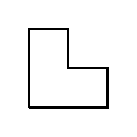
\begin{tikzpicture}
\draw[thick] (0,0) -- (1,0) -- (1,0.5) --(0.5,0.5) -- (0.5,1) -- (0,1) -- (0,0);
\end{tikzpicture}
\end{center}
\end{minipage}
\hfill\begin{minipage}{0.8\linewidth}
{\it Savet:} Dovoljno je dokazati da ova tvrdnja va\v zi za svaku tablu dimenzija $2^n\times 2^n$ gde $n\in\mathbb N$.
\end{minipage}
}

\ZAD{04.zad.12}{
Dokazati slede\' ce ekvivalencije iskaznih formula:
\begin{enumerate}[(a)]
\item $\neg(p_1\wedge p_2\wedge \cdots\wedge p_n)\equiv \neg p_1\vee\neg p_2\vee \cdots\vee\neg p_n$;
\item $p_1\Rightarrow(p_2\Rightarrow\cdots\Rightarrow(p_n\Rightarrow q)\cdots)\equiv p_1\wedge p_2\wedge\cdots\wedge p_n\Rightarrow q$;
\item $(p_1\Rightarrow p_2)\wedge(p_2\Rightarrow p_3)\wedge \cdots\wedge(p_{n-1}\Rightarrow p_n)\models p_1\Rightarrow p_n$.
\end{enumerate}
}

\ZAD{04.zad.13}{
Dokazati da $n$ pravih od kojih se svake dve seku, i od kojih se nikoje tri ne seku u istoj ta\v cki, dele ravan na $\frac{n^2+n+2}2$ delova.

{\it Savet:} Dodavati jednu po jednu pravu, i primetiti za koliko se u svakom koraku pove\' cava broj delova na koje je podeljena ravan.
}

\ZAD{04.zad.14}{
Dokazati da je
\[1+\frac 12+\frac 14+\cdots+\frac 1{2^n}<2\]
za svako $n\in\mathbb N$.

{\it Savet:} Dokazati da je za svako $n\in\mathbb N$
\[1+\frac 12+\frac 14+\cdots+\frac 1{2^n}=2-\frac 1{2^n}.\]
}

%\ZAD{04.zad.15}{
%Dokazati De Moavrovu teoremu:
%$$(\cos\theta+i\sin\theta)^n=\cos(n\theta)+i\sin(n\theta).$$
%{\it Savet:} Iskoristiti adicione formule:
%\begin{align*}
%&\cos(\alpha+\beta)=\cos\alpha\cos\beta-\sin\alpha\sin\alpha\\
%&\sin(\alpha+\beta)=\sin\alpha\cos\beta+\cos\alpha\sin\beta
%\end{align*}
%}

%\ZAD{04.zad.16}{
%Dokazati da je:
%\[\sin\theta+\sin(3\theta)+\cdots+\sin((2n-1)\theta)=\frac{\sin^2(n\theta)}{\sin\theta}\]
%za svako $n\in\mathbb N$ i za svako $\theta$ za koje je $\sin\theta\neq 0$.
%}

%\ZAD{04.zad.17}{
%Dokazati da se svaki prirodan broj $n\geq 2$ mo\v ze zapisati kao proizvod prostih brojeva.
%}
%
%\ZAD{04.zad.18}{
%Dokazati da prostih brojeva ima beskona\v cno mnogo.
%}

\ZAD{04.zad.19}{
Jocina po\v starina je bar 8 centi. Dokazati da on mo\v ze platiti ta\v can iznos svoje po\v starine markicama od 3 i od 5 centi.
}\label{Joca-sa-postarinom}

\ZAD{04.zad.20}{
Bankomat Vasine banke ispla\' cuje nov\v canice od 2000 dinara i od 5000 dinara. Vasa \v zeli da podigne nekoliko hiljada dinara, ali ne manje od \v cetiri hiljade. Dokazati da on mo\v ze da podigne na bankomatu svoje banke ta\v cno koliko \v zeli novca.
}

\ZAD{04.zad.21}{
Ivica sla\v ze slagalicu. Slagalica se sla\v ze tako \v sto se spajaju dva deli\' ca slagalice tako da oni sa\v cine blok, dodavanjem komada slagalice ve\' cem bloku, ili spajanjem dva bloka. Ako Ivi\v cina slagalica ima 500 deli\' ca, dokazati da \' ce je Ivica slo\v ziti u 499 koraka. 
}



\endinput
%%%%%%%%%%%%%%%%%%%%%%%%%%%%%%%%%%%%%%%%%%%%%%%%%

ZADACI:

Svaki broj se mo\v ze zapisati kao zbir razli\v citih stepena broja~2.

Neka je niz $a_1, a_2, a_3, \ldots$ celih brojeva definisan ovako:
$$
  a_1 = 1, a_2 = 2, a_3 = 3, a_n = a_{n-1} + a_{n-2} + a_{n-3}$. Dokazati da je $a_n < 2^n$ za sve $n$.
$$

Neka je niz $a_1, a_2, a_3, \ldots$ celih brojeva definisan ovako:
$$
  a_1 = 1, a_2 = 3, a_3 = 7, a_n = a_{n-1} + a_{n-2} + a_{n-3}$. Dokazati da su svi $a_n$ neparni.
$$















